\documentclass[twoside]{book}

% Packages required by doxygen
\usepackage{calc}
\usepackage{doxygen}
\usepackage{graphicx}
\usepackage[utf8]{inputenc}
\usepackage{makeidx}
\usepackage{multicol}
\usepackage{multirow}
\usepackage{textcomp}
\usepackage[table]{xcolor}

% Font selection
\usepackage[T1]{fontenc}
\usepackage{mathptmx}
\usepackage[scaled=.90]{helvet}
\usepackage{courier}
\usepackage{amssymb}
\usepackage{sectsty}
\renewcommand{\familydefault}{\sfdefault}
\allsectionsfont{%
  \fontseries{bc}\selectfont%
  \color{darkgray}%
}
\renewcommand{\DoxyLabelFont}{%
  \fontseries{bc}\selectfont%
  \color{darkgray}%
}

% Page & text layout
\usepackage{geometry}
\geometry{%
  a4paper,%
  top=2.5cm,%
  bottom=2.5cm,%
  left=2.5cm,%
  right=2.5cm%
}
\tolerance=750
\hfuzz=15pt
\hbadness=750
\setlength{\emergencystretch}{15pt}
\setlength{\parindent}{0cm}
\setlength{\parskip}{0.2cm}
\makeatletter
\renewcommand{\paragraph}{%
  \@startsection{paragraph}{4}{0ex}{-1.0ex}{1.0ex}{%
    \normalfont\normalsize\bfseries\SS@parafont%
  }%
}
\renewcommand{\subparagraph}{%
  \@startsection{subparagraph}{5}{0ex}{-1.0ex}{1.0ex}{%
    \normalfont\normalsize\bfseries\SS@subparafont%
  }%
}
\makeatother

% Headers & footers
\usepackage{fancyhdr}
\pagestyle{fancyplain}
\fancyhead[LE]{\fancyplain{}{\bfseries\thepage}}
\fancyhead[CE]{\fancyplain{}{}}
\fancyhead[RE]{\fancyplain{}{\bfseries\leftmark}}
\fancyhead[LO]{\fancyplain{}{\bfseries\rightmark}}
\fancyhead[CO]{\fancyplain{}{}}
\fancyhead[RO]{\fancyplain{}{\bfseries\thepage}}
\fancyfoot[LE]{\fancyplain{}{}}
\fancyfoot[CE]{\fancyplain{}{}}
\fancyfoot[RE]{\fancyplain{}{\bfseries\scriptsize Generated on Fri Jan 20 2017 23\-:39\-:42 for Ao\-Shared\-Service\-Library by Doxygen }}
\fancyfoot[LO]{\fancyplain{}{\bfseries\scriptsize Generated on Fri Jan 20 2017 23\-:39\-:42 for Ao\-Shared\-Service\-Library by Doxygen }}
\fancyfoot[CO]{\fancyplain{}{}}
\fancyfoot[RO]{\fancyplain{}{}}
\renewcommand{\footrulewidth}{0.4pt}
\renewcommand{\chaptermark}[1]{%
  \markboth{#1}{}%
}
\renewcommand{\sectionmark}[1]{%
  \markright{\thesection\ #1}%
}

% Indices & bibliography
\usepackage{natbib}
\usepackage[titles]{tocloft}
\setcounter{tocdepth}{3}
\setcounter{secnumdepth}{5}
\makeindex

% Hyperlinks (required, but should be loaded last)
\usepackage{ifpdf}
\ifpdf
  \usepackage[pdftex,pagebackref=true]{hyperref}
\else
  \usepackage[ps2pdf,pagebackref=true]{hyperref}
\fi
\hypersetup{%
  colorlinks=true,%
  linkcolor=blue,%
  citecolor=blue,%
  unicode%
}

% Custom commands
\newcommand{\clearemptydoublepage}{%
  \newpage{\pagestyle{empty}\cleardoublepage}%
}


%===== C O N T E N T S =====

\begin{document}

% Titlepage & ToC
\hypersetup{pageanchor=false}
\pagenumbering{roman}
\begin{titlepage}
\vspace*{7cm}
\begin{center}%
{\Large Ao\-Shared\-Service\-Library }\\
\vspace*{1cm}
{\large Generated by Doxygen 1.8.5}\\
\vspace*{0.5cm}
{\small Fri Jan 20 2017 23:39:42}\\
\end{center}
\end{titlepage}
\clearemptydoublepage
\tableofcontents
\clearemptydoublepage
\pagenumbering{arabic}
\hypersetup{pageanchor=true}

%--- Begin generated contents ---
\chapter{Hierarchical Index}
\section{Class Hierarchy}
This inheritance list is sorted roughly, but not completely, alphabetically\+:\begin{DoxyCompactList}
\item \contentsline{section}{Command\+Line\+Interface}{\pageref{classCommandLineInterface}}{}
\item \contentsline{section}{Command\+Line\+Interpreter\+Factory}{\pageref{classCommandLineInterpreterFactory}}{}
\item \contentsline{section}{Consul\+Component\+Factory}{\pageref{classConsulComponentFactory}}{}
\item \contentsline{section}{Consul\+Interface}{\pageref{classConsulInterface}}{}
\item \contentsline{section}{Db\+List\+Interface}{\pageref{classDbListInterface}}{}
\item \contentsline{section}{Db\+Map\+Interface}{\pageref{classDbMapInterface}}{}
\item \contentsline{section}{Db\+Object\+Interface}{\pageref{classDbObjectInterface}}{}
\item exception\begin{DoxyCompactList}
\item \contentsline{section}{Http\+Request\+Exception}{\pageref{structHttpRequestException}}{}
\item \contentsline{section}{Logging\+Exception}{\pageref{structLoggingException}}{}
\item \contentsline{section}{Mongo\+Exception}{\pageref{structMongoException}}{}
\item \contentsline{section}{Redis\+Connection\+Exception}{\pageref{structRedisConnectionException}}{}
\item \contentsline{section}{Redis\+Operation\+Exception}{\pageref{structRedisOperationException}}{}
\end{DoxyCompactList}
\item \contentsline{section}{Health\+Check}{\pageref{structHealthCheck}}{}
\item \contentsline{section}{Http\+Client\+Factory}{\pageref{classHttpClientFactory}}{}
\item \contentsline{section}{Http\+Interface}{\pageref{classHttpInterface}}{}
\item \contentsline{section}{Http\+Server\+Factory}{\pageref{classHttpServerFactory}}{}
\item \contentsline{section}{Http\+Server\+Interface}{\pageref{classHttpServerInterface}}{}
\item \contentsline{section}{Logging\+Category\+Interface}{\pageref{classLoggingCategoryInterface}}{}
\item \contentsline{section}{Logging\+Component\+Factory}{\pageref{classLoggingComponentFactory}}{}
\item \contentsline{section}{Logging\+Interface}{\pageref{classLoggingInterface}}{}
\item \contentsline{section}{Mongo\+Component\+Factory}{\pageref{classMongoComponentFactory}}{}
\item \contentsline{section}{Mongo\+Interface}{\pageref{classMongoInterface}}{}
\item \contentsline{section}{Mongo\+Iterator\+Interface}{\pageref{classMongoIteratorInterface}}{}
\item \contentsline{section}{Mongo\+Response\+Interface}{\pageref{classMongoResponseInterface}}{}
\item \contentsline{section}{Neo4j\+Component\+Factory}{\pageref{classNeo4jComponentFactory}}{}
\item \contentsline{section}{Neo4j\+Interface}{\pageref{classNeo4jInterface}}{}
\item \contentsline{section}{Neo4j\+Query\+Parameter\+Interface}{\pageref{classNeo4jQueryParameterInterface}}{}
\item \contentsline{section}{Properties\+Reader\+Interface}{\pageref{classPropertiesReaderInterface}}{}
\item \contentsline{section}{Property\+Reader\+Factory}{\pageref{classPropertyReaderFactory}}{}
\item \contentsline{section}{Redis\+Component\+Factory}{\pageref{classRedisComponentFactory}}{}
\item \contentsline{section}{Redis\+Conn\+Chain}{\pageref{structRedisConnChain}}{}
\item \contentsline{section}{Redis\+Interface}{\pageref{classRedisInterface}}{}
\item \contentsline{section}{Redis\+Kv\+Pair}{\pageref{structRedisKvPair}}{}
\item \contentsline{section}{Results\+Iterator\+Interface}{\pageref{classResultsIteratorInterface}}{}
\item \contentsline{section}{Result\+Tree\+Interface}{\pageref{classResultTreeInterface}}{}
\item \contentsline{section}{Service\+Interface}{\pageref{classServiceInterface}}{}
\item \contentsline{section}{uuid\+Component\+Factory}{\pageref{classuuidComponentFactory}}{}
\item \contentsline{section}{Uuid\+Container}{\pageref{structUuidContainer}}{}
\item \contentsline{section}{uuid\+Interface}{\pageref{classuuidInterface}}{}
\item \contentsline{section}{Zmq\+Component\+Factory}{\pageref{classZmqComponentFactory}}{}
\item \contentsline{section}{Zmqio}{\pageref{classZmqio}}{}
\begin{DoxyCompactList}
\item \contentsline{section}{Zmq\+In}{\pageref{classZmqIn}}{}
\item \contentsline{section}{Zmq\+Out}{\pageref{classZmqOut}}{}
\end{DoxyCompactList}
\end{DoxyCompactList}

\chapter{Class Index}
\section{Class List}
Here are the classes, structs, unions and interfaces with brief descriptions\-:\begin{DoxyCompactList}
\item\contentsline{section}{\hyperlink{classCommandLineInterface}{Command\-Line\-Interface} \\*\hyperlink{classCommandLineInterface}{Command\-Line\-Interface} }{\pageref{classCommandLineInterface}}{}
\item\contentsline{section}{\hyperlink{classConsulInterface}{Consul\-Interface} \\*The Consul Administrator, who handles distributed configuration \& service discovery }{\pageref{classConsulInterface}}{}
\item\contentsline{section}{\hyperlink{structCouchbaseBootstrapException}{Couchbase\-Bootstrap\-Exception} \\*An Implementation of std\-::exception that denotes an error in Couchbase during bootstrap }{\pageref{structCouchbaseBootstrapException}}{}
\item\contentsline{section}{\hyperlink{structCouchbaseConnectException}{Couchbase\-Connect\-Exception} \\*An Implementation of std\-::exception that denotes an error connecting to Couchbase }{\pageref{structCouchbaseConnectException}}{}
\item\contentsline{section}{\hyperlink{structCouchbaseInitException}{Couchbase\-Init\-Exception} \\*An Implementation of std\-::exception that denotes an error in Couchbase during initialization of the client library }{\pageref{structCouchbaseInitException}}{}
\item\contentsline{section}{\hyperlink{classCouchbaseInterface}{Couchbase\-Interface} \\*The Couchbase Administrator handles interactions with the Couchbase D\-B }{\pageref{classCouchbaseInterface}}{}
\item\contentsline{section}{\hyperlink{structCouchbaseOperationException}{Couchbase\-Operation\-Exception} \\*An Implementation of std\-::exception that denotes an error in Couchbase during a transaction }{\pageref{structCouchbaseOperationException}}{}
\item\contentsline{section}{\hyperlink{classDBAdmin}{D\-B\-Admin} \\*Database Administrator Interface }{\pageref{classDBAdmin}}{}
\item\contentsline{section}{\hyperlink{classDbListInterface}{Db\-List\-Interface} \\*A Neo4j List }{\pageref{classDbListInterface}}{}
\item\contentsline{section}{\hyperlink{classDbMapInterface}{Db\-Map\-Interface} \\*A Neo4j Map }{\pageref{classDbMapInterface}}{}
\item\contentsline{section}{\hyperlink{classDbObjectInterface}{Db\-Object\-Interface} \\*A Neo4j Object }{\pageref{classDbObjectInterface}}{}
\item\contentsline{section}{\hyperlink{structHealthCheck}{Health\-Check} \\*A struct to hold health check information which can be added to a service }{\pageref{structHealthCheck}}{}
\item\contentsline{section}{\hyperlink{classHttpInterface}{Http\-Interface} \\*The H\-T\-T\-P Requests Administrators }{\pageref{classHttpInterface}}{}
\item\contentsline{section}{\hyperlink{structHttpRequestException}{Http\-Request\-Exception} \\*An Implementation of std\-::exception that denotes an error in Couchbase during bootstrap }{\pageref{structHttpRequestException}}{}
\item\contentsline{section}{\hyperlink{classHttpServerInterface}{Http\-Server\-Interface} \\*This is a basic H\-T\-T\-P Server that can be used to build a R\-E\-S\-Tful A\-P\-I }{\pageref{classHttpServerInterface}}{}
\item\contentsline{section}{\hyperlink{classInterpreter}{Interpreter} \\*\hyperlink{classInterpreter}{Interpreter} Interface }{\pageref{classInterpreter}}{}
\item\contentsline{section}{\hyperlink{classLoggingCategoryInterface}{Logging\-Category\-Interface} \\*A Logging Category instantiated on a standard logging instance }{\pageref{classLoggingCategoryInterface}}{}
\item\contentsline{section}{\hyperlink{classLoggingInterface}{Logging\-Interface} \\*An overall logging interface, which can generate logging categories }{\pageref{classLoggingInterface}}{}
\item\contentsline{section}{\hyperlink{structMongoException}{Mongo\-Exception} }{\pageref{structMongoException}}{}
\item\contentsline{section}{\hyperlink{classMongoInterface}{Mongo\-Interface} }{\pageref{classMongoInterface}}{}
\item\contentsline{section}{\hyperlink{structNeo4jException}{Neo4j\-Exception} \\*A Neo4j Exception }{\pageref{structNeo4jException}}{}
\item\contentsline{section}{\hyperlink{classNeo4jInterface}{Neo4j\-Interface} \\*Neo4j Query Interface }{\pageref{classNeo4jInterface}}{}
\item\contentsline{section}{\hyperlink{classPropertiesReaderInterface}{Properties\-Reader\-Interface} \\*\hyperlink{classPropertiesReaderInterface}{Properties\-Reader\-Interface} }{\pageref{classPropertiesReaderInterface}}{}
\item\contentsline{section}{\hyperlink{structRedisConnChain}{Redis\-Conn\-Chain} \\*A Structure for storing Redis Connection Information }{\pageref{structRedisConnChain}}{}
\item\contentsline{section}{\hyperlink{structRedisConnectionException}{Redis\-Connection\-Exception} \\*An Implementation of std\-::exception that denotes a connection error within Redis }{\pageref{structRedisConnectionException}}{}
\item\contentsline{section}{\hyperlink{classRedisInterface}{Redis\-Interface} \\*The Redis Admin }{\pageref{classRedisInterface}}{}
\item\contentsline{section}{\hyperlink{structRedisKvPair}{Redis\-Kv\-Pair} \\*A Structure for storing a Key-\/\-Value pair, used with batch operations }{\pageref{structRedisKvPair}}{}
\item\contentsline{section}{\hyperlink{structRedisOperationException}{Redis\-Operation\-Exception} \\*An Implementation of std\-::exception that denotes an error within Redis during a transaction }{\pageref{structRedisOperationException}}{}
\item\contentsline{section}{\hyperlink{structRequest}{Request} \\*A struct that gets passed to callbacks }{\pageref{structRequest}}{}
\item\contentsline{section}{\hyperlink{structRequestError}{Request\-Error} \\*A struct that gets passed to callbacks to transmit errors }{\pageref{structRequestError}}{}
\item\contentsline{section}{\hyperlink{classResultsIteratorInterface}{Results\-Iterator\-Interface} \\*Results Iterator for viewing query results }{\pageref{classResultsIteratorInterface}}{}
\item\contentsline{section}{\hyperlink{classResultTreeInterface}{Result\-Tree\-Interface} \\*Tree of Query Results }{\pageref{classResultTreeInterface}}{}
\item\contentsline{section}{\hyperlink{classServiceInterface}{Service\-Interface} \\*A Service class which can be registered with Consul for each instance of a particular service }{\pageref{classServiceInterface}}{}
\item\contentsline{section}{\hyperlink{structUuidContainer}{Uuid\-Container} \\*A return structure which captures any security error messages thrown by the framework }{\pageref{structUuidContainer}}{}
\item\contentsline{section}{\hyperlink{classuuidInterface}{uuid\-Interface} \\*U\-U\-I\-D Admin }{\pageref{classuuidInterface}}{}
\item\contentsline{section}{\hyperlink{classWriteable}{Writeable} \\*The \hyperlink{classWriteable}{Writeable} Interface }{\pageref{classWriteable}}{}
\item\contentsline{section}{\hyperlink{classZmqIn}{Zmq\-In} \\*An Inbound Z\-M\-Q Manager }{\pageref{classZmqIn}}{}
\item\contentsline{section}{\hyperlink{classZmqio}{Zmqio} \\*An Interface for Z\-M\-Q\-I\-O }{\pageref{classZmqio}}{}
\item\contentsline{section}{\hyperlink{classZmqOut}{Zmq\-Out} \\*An Outbound Z\-M\-Q Manager }{\pageref{classZmqOut}}{}
\end{DoxyCompactList}

\chapter{Class Documentation}
\hypertarget{classCommandLineInterface}{}\section{Command\+Line\+Interface Class Reference}
\label{classCommandLineInterface}\index{Command\+Line\+Interface@{Command\+Line\+Interface}}


\hyperlink{classCommandLineInterface}{Command\+Line\+Interface}.  




{\ttfamily \#include $<$commandline\+\_\+interface.\+h$>$}

\subsection*{Public Member Functions}
\begin{DoxyCompactItemize}
\item 
virtual bool \hyperlink{classCommandLineInterface_a4ee445b7c34f27b7fc9d265d88e5d82a}{opt\+\_\+exist} (std\+::string key)=0\hypertarget{classCommandLineInterface_a4ee445b7c34f27b7fc9d265d88e5d82a}{}\label{classCommandLineInterface_a4ee445b7c34f27b7fc9d265d88e5d82a}

\begin{DoxyCompactList}\small\item\em Does a key exist? \end{DoxyCompactList}\item 
virtual std\+::string \hyperlink{classCommandLineInterface_a12399397b591b0eb779caad05947f800}{get\+\_\+opt} (std\+::string key)=0\hypertarget{classCommandLineInterface_a12399397b591b0eb779caad05947f800}{}\label{classCommandLineInterface_a12399397b591b0eb779caad05947f800}

\begin{DoxyCompactList}\small\item\em Get an option by key. \end{DoxyCompactList}\item 
virtual std\+::string \hyperlink{classCommandLineInterface_a47bd2a11bc8d8f507a7f75dbef36a3c9}{get\+\_\+program\+\_\+name} ()=0
\begin{DoxyCompactList}\small\item\em Get the program name. \end{DoxyCompactList}\end{DoxyCompactItemize}


\subsection{Detailed Description}
\hyperlink{classCommandLineInterface}{Command\+Line\+Interface}. 

Here we create a new interpreter by passing in the two arguments from the main method, int argc \& char$\ast$ argv\mbox{[}\mbox{]}. This parses arguments passed in the form\+: -\/arg\+\_\+key=arg\+\_\+val 

\subsection{Member Function Documentation}
\index{Command\+Line\+Interface@{Command\+Line\+Interface}!get\+\_\+program\+\_\+name@{get\+\_\+program\+\_\+name}}
\index{get\+\_\+program\+\_\+name@{get\+\_\+program\+\_\+name}!Command\+Line\+Interface@{Command\+Line\+Interface}}
\subsubsection[{\texorpdfstring{get\+\_\+program\+\_\+name()=0}{get_program_name()=0}}]{\setlength{\rightskip}{0pt plus 5cm}virtual std\+::string Command\+Line\+Interface\+::get\+\_\+program\+\_\+name (
\begin{DoxyParamCaption}
{}
\end{DoxyParamCaption}
)\hspace{0.3cm}{\ttfamily [pure virtual]}}\hypertarget{classCommandLineInterface_a47bd2a11bc8d8f507a7f75dbef36a3c9}{}\label{classCommandLineInterface_a47bd2a11bc8d8f507a7f75dbef36a3c9}


Get the program name. 

Get the name of the executable currently being run. 

The documentation for this class was generated from the following file\+:\begin{DoxyCompactItemize}
\item 
aossl/commandline/include/commandline\+\_\+interface.\+h\end{DoxyCompactItemize}

\hypertarget{classConsulInterface}{}\section{Consul\+Interface Class Reference}
\label{classConsulInterface}\index{Consul\+Interface@{Consul\+Interface}}


The Consul Administrator, who handles distributed configuration \& service discovery.  




{\ttfamily \#include $<$consul\+\_\+interface.\+h$>$}

\subsection*{Public Member Functions}
\begin{DoxyCompactItemize}
\item 
virtual std\+::string \hyperlink{classConsulInterface_a636b134672f2c150f6b38fc821fb2348}{base64\+\_\+decode} (std\+::string const \&encoded\+\_\+string)=0
\begin{DoxyCompactList}\small\item\em Convinience Method for base64 decoding. \end{DoxyCompactList}\item 
virtual bool \hyperlink{classConsulInterface_ad1d3a241b2fc31e4b13789a49a0d010a}{register\+\_\+service} (\hyperlink{classServiceInterface}{Service\+Interface} \&s)=0\hypertarget{classConsulInterface_ad1d3a241b2fc31e4b13789a49a0d010a}{}\label{classConsulInterface_ad1d3a241b2fc31e4b13789a49a0d010a}

\begin{DoxyCompactList}\small\item\em Register the Service. \end{DoxyCompactList}\item 
virtual bool \hyperlink{classConsulInterface_ac97f7a426f3de5023edc637ab984b4c4}{deregister\+\_\+service} (\hyperlink{classServiceInterface}{Service\+Interface} \&s)=0\hypertarget{classConsulInterface_ac97f7a426f3de5023edc637ab984b4c4}{}\label{classConsulInterface_ac97f7a426f3de5023edc637ab984b4c4}

\begin{DoxyCompactList}\small\item\em Deregister the Service. \end{DoxyCompactList}\item 
virtual bool \hyperlink{classConsulInterface_a98ce2623db59b3f8804691a4039957a8}{set\+\_\+config\+\_\+value} (std\+::string key, std\+::string val)=0
\begin{DoxyCompactList}\small\item\em Set a configuration value. \end{DoxyCompactList}\item 
virtual std\+::string \hyperlink{classConsulInterface_a1cc4bdfe75f86f69626e109847aba6af}{get\+\_\+config\+\_\+value} (std\+::string key)=0\hypertarget{classConsulInterface_a1cc4bdfe75f86f69626e109847aba6af}{}\label{classConsulInterface_a1cc4bdfe75f86f69626e109847aba6af}

\begin{DoxyCompactList}\small\item\em Get a configuration value. \end{DoxyCompactList}\item 
virtual bool \hyperlink{classConsulInterface_a3a6e57ac45cf284e92def6136b0e23d9}{del\+\_\+config\+\_\+value} (std\+::string key)=0\hypertarget{classConsulInterface_a3a6e57ac45cf284e92def6136b0e23d9}{}\label{classConsulInterface_a3a6e57ac45cf284e92def6136b0e23d9}

\begin{DoxyCompactList}\small\item\em Delete a configuration value. \end{DoxyCompactList}\item 
virtual std\+::string \hyperlink{classConsulInterface_ad130a602282f9854a2eae856bb60a745}{services} ()=0\hypertarget{classConsulInterface_ad130a602282f9854a2eae856bb60a745}{}\label{classConsulInterface_ad130a602282f9854a2eae856bb60a745}

\begin{DoxyCompactList}\small\item\em Query the local agent for services registered. \end{DoxyCompactList}\item 
virtual std\+::string \hyperlink{classConsulInterface_a6fb0bda867b267614b44328fd044859e}{agent\+\_\+info} ()=0\hypertarget{classConsulInterface_a6fb0bda867b267614b44328fd044859e}{}\label{classConsulInterface_a6fb0bda867b267614b44328fd044859e}

\begin{DoxyCompactList}\small\item\em Query the local agent for it\textquotesingle{}s info. \end{DoxyCompactList}\item 
virtual std\+::string \hyperlink{classConsulInterface_a229eaac89811b9e1f5f3c9ec70ea68aa}{healthy\+\_\+services} ()=0\hypertarget{classConsulInterface_a229eaac89811b9e1f5f3c9ec70ea68aa}{}\label{classConsulInterface_a229eaac89811b9e1f5f3c9ec70ea68aa}

\begin{DoxyCompactList}\small\item\em Query for healthy services only. \end{DoxyCompactList}\item 
virtual std\+::string \hyperlink{classConsulInterface_a16848fcc856afae488c55e4f4febf268}{datacenters} ()=0\hypertarget{classConsulInterface_a16848fcc856afae488c55e4f4febf268}{}\label{classConsulInterface_a16848fcc856afae488c55e4f4febf268}

\begin{DoxyCompactList}\small\item\em Query the catalog for datacenters. \end{DoxyCompactList}\item 
virtual std\+::string \hyperlink{classConsulInterface_a0831246af1b80ce5bbe074a47333c615}{nodes\+\_\+dc} (std\+::string data\+\_\+center)=0\hypertarget{classConsulInterface_a0831246af1b80ce5bbe074a47333c615}{}\label{classConsulInterface_a0831246af1b80ce5bbe074a47333c615}

\begin{DoxyCompactList}\small\item\em Query the catalog for the nodes in a particular datacenter. \end{DoxyCompactList}\item 
virtual std\+::string \hyperlink{classConsulInterface_ab1c3f2169a8aebdb5a66cfe8211330dc}{services\+\_\+dc} (std\+::string data\+\_\+center)=0\hypertarget{classConsulInterface_ab1c3f2169a8aebdb5a66cfe8211330dc}{}\label{classConsulInterface_ab1c3f2169a8aebdb5a66cfe8211330dc}

\begin{DoxyCompactList}\small\item\em Query the catalog for the services in a particular datacenter. \end{DoxyCompactList}\item 
virtual std\+::string \hyperlink{classConsulInterface_a7490a960b2e10855c7d7ff09d87942b8}{nodes\+\_\+service} (std\+::string service)=0\hypertarget{classConsulInterface_a7490a960b2e10855c7d7ff09d87942b8}{}\label{classConsulInterface_a7490a960b2e10855c7d7ff09d87942b8}

\begin{DoxyCompactList}\small\item\em Query the catalog for the nodes running a particular service. \end{DoxyCompactList}\item 
virtual std\+::string \hyperlink{classConsulInterface_abbd5b2839d3548d48e93074a53844f40}{services\+\_\+node} (std\+::string node, std\+::string data\+\_\+center)=0\hypertarget{classConsulInterface_abbd5b2839d3548d48e93074a53844f40}{}\label{classConsulInterface_abbd5b2839d3548d48e93074a53844f40}

\begin{DoxyCompactList}\small\item\em Query the catalog for the services provided by a particular node. \end{DoxyCompactList}\end{DoxyCompactItemize}


\subsection{Detailed Description}
The Consul Administrator, who handles distributed configuration \& service discovery. 

This relies on the H\+T\+TP Administrator, and takes in a Service object in order to register. It\textquotesingle{}s responses are J\+S\+ON strings that are recieved from Consul. Note that the values returned from the Key-\/\+Value store will be stored in base64 format 

\subsection{Member Function Documentation}
\index{Consul\+Interface@{Consul\+Interface}!base64\+\_\+decode@{base64\+\_\+decode}}
\index{base64\+\_\+decode@{base64\+\_\+decode}!Consul\+Interface@{Consul\+Interface}}
\subsubsection[{\texorpdfstring{base64\+\_\+decode(std\+::string const \&encoded\+\_\+string)=0}{base64_decode(std::string const &encoded_string)=0}}]{\setlength{\rightskip}{0pt plus 5cm}virtual std\+::string Consul\+Interface\+::base64\+\_\+decode (
\begin{DoxyParamCaption}
\item[{std\+::string const \&}]{encoded\+\_\+string}
\end{DoxyParamCaption}
)\hspace{0.3cm}{\ttfamily [pure virtual]}}\hypertarget{classConsulInterface_a636b134672f2c150f6b38fc821fb2348}{}\label{classConsulInterface_a636b134672f2c150f6b38fc821fb2348}


Convinience Method for base64 decoding. 

This is needed as all configuration values are returned from Consul in base64, and need to be decoded after the json is parsed. \index{Consul\+Interface@{Consul\+Interface}!set\+\_\+config\+\_\+value@{set\+\_\+config\+\_\+value}}
\index{set\+\_\+config\+\_\+value@{set\+\_\+config\+\_\+value}!Consul\+Interface@{Consul\+Interface}}
\subsubsection[{\texorpdfstring{set\+\_\+config\+\_\+value(std\+::string key, std\+::string val)=0}{set_config_value(std::string key, std::string val)=0}}]{\setlength{\rightskip}{0pt plus 5cm}virtual bool Consul\+Interface\+::set\+\_\+config\+\_\+value (
\begin{DoxyParamCaption}
\item[{std\+::string}]{key, }
\item[{std\+::string}]{val}
\end{DoxyParamCaption}
)\hspace{0.3cm}{\ttfamily [pure virtual]}}\hypertarget{classConsulInterface_a98ce2623db59b3f8804691a4039957a8}{}\label{classConsulInterface_a98ce2623db59b3f8804691a4039957a8}


Set a configuration value. 

If the key does not exist, then this will add it. Otherwise, it will update the existing key. 

The documentation for this class was generated from the following file\+:\begin{DoxyCompactItemize}
\item 
aossl/consul/include/consul\+\_\+interface.\+h\end{DoxyCompactItemize}

\hypertarget{classDbListInterface}{\section{Db\-List\-Interface Class Reference}
\label{classDbListInterface}\index{Db\-List\-Interface@{Db\-List\-Interface}}
}


A Neo4j List.  




{\ttfamily \#include $<$neo4j\-\_\-interface.\-h$>$}

\subsection*{Public Member Functions}
\begin{DoxyCompactItemize}
\item 
\hypertarget{classDbListInterface_af08cd8eb6763d9963e8ba359d0139fab}{virtual \hyperlink{classDbListInterface}{Db\-List\-Interface} $\ast$ \hyperlink{classDbListInterface_af08cd8eb6763d9963e8ba359d0139fab}{get\-\_\-list\-\_\-element} (unsigned int ind)=0}\label{classDbListInterface_af08cd8eb6763d9963e8ba359d0139fab}

\begin{DoxyCompactList}\small\item\em Get a list element out of a list. \end{DoxyCompactList}\item 
\hypertarget{classDbListInterface_aed51c97a5b72e67402d750bf8540b7b4}{virtual bool \hyperlink{classDbListInterface_aed51c97a5b72e67402d750bf8540b7b4}{get\-\_\-bool\-\_\-element} (unsigned int ind)=0}\label{classDbListInterface_aed51c97a5b72e67402d750bf8540b7b4}

\begin{DoxyCompactList}\small\item\em Get a bool element out of a list. \end{DoxyCompactList}\item 
\hypertarget{classDbListInterface_a21aa8acc708256af0e5b81f264961ab5}{virtual int \hyperlink{classDbListInterface_a21aa8acc708256af0e5b81f264961ab5}{get\-\_\-int\-\_\-element} (unsigned int ind)=0}\label{classDbListInterface_a21aa8acc708256af0e5b81f264961ab5}

\begin{DoxyCompactList}\small\item\em Get an int element out of a list. \end{DoxyCompactList}\item 
\hypertarget{classDbListInterface_aa14ef83f3dd278197d0b36a2c41fb097}{virtual float \hyperlink{classDbListInterface_aa14ef83f3dd278197d0b36a2c41fb097}{get\-\_\-float\-\_\-element} (unsigned int ind)=0}\label{classDbListInterface_aa14ef83f3dd278197d0b36a2c41fb097}

\begin{DoxyCompactList}\small\item\em Get a float element out of a list. \end{DoxyCompactList}\item 
\hypertarget{classDbListInterface_ac30844705b9358941448b5ee3db91542}{virtual std\-::string \hyperlink{classDbListInterface_ac30844705b9358941448b5ee3db91542}{get\-\_\-string\-\_\-element} (unsigned int ind, int char\-\_\-buffer\-\_\-size)=0}\label{classDbListInterface_ac30844705b9358941448b5ee3db91542}

\begin{DoxyCompactList}\small\item\em Get a list string out of a list. \end{DoxyCompactList}\item 
\hypertarget{classDbListInterface_a5b56c68ef216efd371e17d65ad6adee1}{virtual std\-::string \hyperlink{classDbListInterface_a5b56c68ef216efd371e17d65ad6adee1}{get\-\_\-string\-\_\-element} (unsigned int ind)=0}\label{classDbListInterface_a5b56c68ef216efd371e17d65ad6adee1}

\begin{DoxyCompactList}\small\item\em Get a string element out of a list. \end{DoxyCompactList}\item 
\hypertarget{classDbListInterface_a18c8fd940cf2225ef9417e2b54ed0fe2}{virtual std\-::string \hyperlink{classDbListInterface_a18c8fd940cf2225ef9417e2b54ed0fe2}{to\-\_\-string} ()=0}\label{classDbListInterface_a18c8fd940cf2225ef9417e2b54ed0fe2}

\begin{DoxyCompactList}\small\item\em Get the string representation of the list. \end{DoxyCompactList}\item 
\hypertarget{classDbListInterface_a5e811b296b3bf7cea5149fce6d69138d}{virtual unsigned int \hyperlink{classDbListInterface_a5e811b296b3bf7cea5149fce6d69138d}{size} ()=0}\label{classDbListInterface_a5e811b296b3bf7cea5149fce6d69138d}

\begin{DoxyCompactList}\small\item\em Get the size of a list. \end{DoxyCompactList}\end{DoxyCompactItemize}


\subsection{Detailed Description}
A Neo4j List. 

This is returned for list elements in a map as well as node labels 

The documentation for this class was generated from the following file\-:\begin{DoxyCompactItemize}
\item 
lib/include/factory/neo4j\-\_\-interface.\-h\end{DoxyCompactItemize}

\hypertarget{classDbMapInterface}{\section{Db\-Map\-Interface Class Reference}
\label{classDbMapInterface}\index{Db\-Map\-Interface@{Db\-Map\-Interface}}
}


A Neo4j Map.  




{\ttfamily \#include $<$neo4j\-\_\-interface.\-h$>$}

\subsection*{Public Member Functions}
\begin{DoxyCompactItemize}
\item 
\hypertarget{classDbMapInterface_a56d046e72d1856177adc71a0aaa09952}{virtual unsigned int \hyperlink{classDbMapInterface_a56d046e72d1856177adc71a0aaa09952}{size} ()=0}\label{classDbMapInterface_a56d046e72d1856177adc71a0aaa09952}

\begin{DoxyCompactList}\small\item\em Get the size of the map. \end{DoxyCompactList}\item 
\hypertarget{classDbMapInterface_ae65d2f6aaad50dc9728ba8aeb6cc557f}{virtual std\-::string \hyperlink{classDbMapInterface_ae65d2f6aaad50dc9728ba8aeb6cc557f}{get\-\_\-string\-\_\-element} (std\-::string key, int char\-\_\-buffer\-\_\-size)=0}\label{classDbMapInterface_ae65d2f6aaad50dc9728ba8aeb6cc557f}

\begin{DoxyCompactList}\small\item\em Get a string element out of a map. \end{DoxyCompactList}\item 
\hypertarget{classDbMapInterface_a26cfc56d753345b64fa9ab08b10dac34}{virtual std\-::string \hyperlink{classDbMapInterface_a26cfc56d753345b64fa9ab08b10dac34}{get\-\_\-string\-\_\-element} (std\-::string key)=0}\label{classDbMapInterface_a26cfc56d753345b64fa9ab08b10dac34}

\begin{DoxyCompactList}\small\item\em Get a string element out of a map. \end{DoxyCompactList}\item 
\hypertarget{classDbMapInterface_a402f75085fa2dacc8808d4b3650bd652}{virtual bool \hyperlink{classDbMapInterface_a402f75085fa2dacc8808d4b3650bd652}{get\-\_\-bool\-\_\-element} (std\-::string key)=0}\label{classDbMapInterface_a402f75085fa2dacc8808d4b3650bd652}

\begin{DoxyCompactList}\small\item\em Get a bool element out of a map. \end{DoxyCompactList}\item 
\hypertarget{classDbMapInterface_af64b01be1c5046a7f24ad6ca0679eb2e}{virtual int \hyperlink{classDbMapInterface_af64b01be1c5046a7f24ad6ca0679eb2e}{get\-\_\-int\-\_\-element} (std\-::string key)=0}\label{classDbMapInterface_af64b01be1c5046a7f24ad6ca0679eb2e}

\begin{DoxyCompactList}\small\item\em Get an int element out of a map. \end{DoxyCompactList}\item 
\hypertarget{classDbMapInterface_a7ac207f3a2e80a4817247069465bb6d7}{virtual float \hyperlink{classDbMapInterface_a7ac207f3a2e80a4817247069465bb6d7}{get\-\_\-float\-\_\-element} (std\-::string key)=0}\label{classDbMapInterface_a7ac207f3a2e80a4817247069465bb6d7}

\begin{DoxyCompactList}\small\item\em Get a float element out of a map. \end{DoxyCompactList}\item 
\hypertarget{classDbMapInterface_a4a44768d0cb0aea730ddad18a7be8075}{virtual \hyperlink{classDbMapInterface}{Db\-Map\-Interface} $\ast$ \hyperlink{classDbMapInterface_a4a44768d0cb0aea730ddad18a7be8075}{get\-\_\-map\-\_\-element} (std\-::string key)=0}\label{classDbMapInterface_a4a44768d0cb0aea730ddad18a7be8075}

\begin{DoxyCompactList}\small\item\em Get a map element out of a map. \end{DoxyCompactList}\item 
\hypertarget{classDbMapInterface_aa6cdf8e968d4f5c46e9f24abff10133d}{virtual \hyperlink{classDbListInterface}{Db\-List\-Interface} $\ast$ \hyperlink{classDbMapInterface_aa6cdf8e968d4f5c46e9f24abff10133d}{get\-\_\-list\-\_\-element} (std\-::string key)=0}\label{classDbMapInterface_aa6cdf8e968d4f5c46e9f24abff10133d}

\begin{DoxyCompactList}\small\item\em Get a list element out of a map. \end{DoxyCompactList}\item 
\hypertarget{classDbMapInterface_ad42e26caf01cf8bae0f98db95e32202c}{virtual std\-::string \hyperlink{classDbMapInterface_ad42e26caf01cf8bae0f98db95e32202c}{to\-\_\-string} ()=0}\label{classDbMapInterface_ad42e26caf01cf8bae0f98db95e32202c}

\begin{DoxyCompactList}\small\item\em Get the string representation of the map. \end{DoxyCompactList}\end{DoxyCompactItemize}


\subsection{Detailed Description}
A Neo4j Map. 

This is returned for map elements in a map as well as node/edge properties 

The documentation for this class was generated from the following file\-:\begin{DoxyCompactItemize}
\item 
lib/include/factory/neo4j\-\_\-interface.\-h\end{DoxyCompactItemize}

\hypertarget{classDbObjectInterface}{}\section{Db\+Object\+Interface Class Reference}
\label{classDbObjectInterface}\index{Db\+Object\+Interface@{Db\+Object\+Interface}}


A Neo4j Object.  




{\ttfamily \#include $<$neo4j\+\_\+interface.\+h$>$}

\subsection*{Public Member Functions}
\begin{DoxyCompactItemize}
\item 
virtual bool \hyperlink{classDbObjectInterface_a3c1c9af939a1e038a082930e57c2afca}{is\+\_\+node} ()=0
\begin{DoxyCompactList}\small\item\em Is this a node? \end{DoxyCompactList}\item 
virtual bool \hyperlink{classDbObjectInterface_af2ab883d4af94b4e7bd25a117bb1f39b}{is\+\_\+edge} ()=0
\begin{DoxyCompactList}\small\item\em Is this an edge? \end{DoxyCompactList}\item 
virtual bool \hyperlink{classDbObjectInterface_ad4ec7a23a86d18fea543376dc6bf6c56}{is\+\_\+path} ()=0
\begin{DoxyCompactList}\small\item\em Is this a path? \end{DoxyCompactList}\item 
virtual std\+::string \hyperlink{classDbObjectInterface_a93c98f06ce3f5493525dd19b337cebbc}{to\+\_\+string} ()=0\hypertarget{classDbObjectInterface_a93c98f06ce3f5493525dd19b337cebbc}{}\label{classDbObjectInterface_a93c98f06ce3f5493525dd19b337cebbc}

\begin{DoxyCompactList}\small\item\em Get the string representation of the object. \end{DoxyCompactList}\item 
virtual \hyperlink{classDbMapInterface}{Db\+Map\+Interface} $\ast$ \hyperlink{classDbObjectInterface_aeede7445ae376fc03af884d5b6f1cb2e}{properties} ()=0
\begin{DoxyCompactList}\small\item\em Get the properties of the object. \end{DoxyCompactList}\item 
virtual \hyperlink{classDbListInterface}{Db\+List\+Interface} $\ast$ \hyperlink{classDbObjectInterface_a281232cca6b9f53f3881100b1a7e5915}{labels} ()=0
\begin{DoxyCompactList}\small\item\em Get the labels of the node. \end{DoxyCompactList}\item 
virtual std\+::string \hyperlink{classDbObjectInterface_a9c2f2de3322439ccdc8e16bd98388040}{type} ()=0
\begin{DoxyCompactList}\small\item\em Get the type of the edge. \end{DoxyCompactList}\item 
virtual bool \hyperlink{classDbObjectInterface_aa3c62699db544791329860136732ddde}{forward} ()=0
\begin{DoxyCompactList}\small\item\em Was the edge traversed in it\textquotesingle{}s natural direction? \end{DoxyCompactList}\item 
virtual unsigned int \hyperlink{classDbObjectInterface_a52f1decaf825e88d3f3e977770af58a0}{size} ()=0
\begin{DoxyCompactList}\small\item\em Get the size of the path. \end{DoxyCompactList}\item 
virtual \hyperlink{classDbObjectInterface}{Db\+Object\+Interface} $\ast$ \hyperlink{classDbObjectInterface_ac6e90274f7a162ffc9c49570ff8f69b6}{get\+\_\+path\+\_\+element} (int path\+\_\+index)=0
\begin{DoxyCompactList}\small\item\em Get an element from a path object. \end{DoxyCompactList}\end{DoxyCompactItemize}


\subsection{Detailed Description}
A Neo4j Object. 

This is returned from a result tree and represents either a node, an edge, or a path 

\subsection{Member Function Documentation}
\index{Db\+Object\+Interface@{Db\+Object\+Interface}!forward@{forward}}
\index{forward@{forward}!Db\+Object\+Interface@{Db\+Object\+Interface}}
\subsubsection[{\texorpdfstring{forward()=0}{forward()=0}}]{\setlength{\rightskip}{0pt plus 5cm}virtual bool Db\+Object\+Interface\+::forward (
\begin{DoxyParamCaption}
{}
\end{DoxyParamCaption}
)\hspace{0.3cm}{\ttfamily [pure virtual]}}\hypertarget{classDbObjectInterface_aa3c62699db544791329860136732ddde}{}\label{classDbObjectInterface_aa3c62699db544791329860136732ddde}


Was the edge traversed in it\textquotesingle{}s natural direction? 

This functions only for edge objects which were taken from a Path \index{Db\+Object\+Interface@{Db\+Object\+Interface}!get\+\_\+path\+\_\+element@{get\+\_\+path\+\_\+element}}
\index{get\+\_\+path\+\_\+element@{get\+\_\+path\+\_\+element}!Db\+Object\+Interface@{Db\+Object\+Interface}}
\subsubsection[{\texorpdfstring{get\+\_\+path\+\_\+element(int path\+\_\+index)=0}{get_path_element(int path_index)=0}}]{\setlength{\rightskip}{0pt plus 5cm}virtual {\bf Db\+Object\+Interface}$\ast$ Db\+Object\+Interface\+::get\+\_\+path\+\_\+element (
\begin{DoxyParamCaption}
\item[{int}]{path\+\_\+index}
\end{DoxyParamCaption}
)\hspace{0.3cm}{\ttfamily [pure virtual]}}\hypertarget{classDbObjectInterface_ac6e90274f7a162ffc9c49570ff8f69b6}{}\label{classDbObjectInterface_ac6e90274f7a162ffc9c49570ff8f69b6}


Get an element from a path object. 

Get an element from a path at the specified index. This functions only for path objects \index{Db\+Object\+Interface@{Db\+Object\+Interface}!is\+\_\+edge@{is\+\_\+edge}}
\index{is\+\_\+edge@{is\+\_\+edge}!Db\+Object\+Interface@{Db\+Object\+Interface}}
\subsubsection[{\texorpdfstring{is\+\_\+edge()=0}{is_edge()=0}}]{\setlength{\rightskip}{0pt plus 5cm}virtual bool Db\+Object\+Interface\+::is\+\_\+edge (
\begin{DoxyParamCaption}
{}
\end{DoxyParamCaption}
)\hspace{0.3cm}{\ttfamily [pure virtual]}}\hypertarget{classDbObjectInterface_af2ab883d4af94b4e7bd25a117bb1f39b}{}\label{classDbObjectInterface_af2ab883d4af94b4e7bd25a117bb1f39b}


Is this an edge? 

Return false if this is a node or path object. Return true if this is an edge object. \index{Db\+Object\+Interface@{Db\+Object\+Interface}!is\+\_\+node@{is\+\_\+node}}
\index{is\+\_\+node@{is\+\_\+node}!Db\+Object\+Interface@{Db\+Object\+Interface}}
\subsubsection[{\texorpdfstring{is\+\_\+node()=0}{is_node()=0}}]{\setlength{\rightskip}{0pt plus 5cm}virtual bool Db\+Object\+Interface\+::is\+\_\+node (
\begin{DoxyParamCaption}
{}
\end{DoxyParamCaption}
)\hspace{0.3cm}{\ttfamily [pure virtual]}}\hypertarget{classDbObjectInterface_a3c1c9af939a1e038a082930e57c2afca}{}\label{classDbObjectInterface_a3c1c9af939a1e038a082930e57c2afca}


Is this a node? 

Return true if this is a node object. Return false if this is an edge or path object. \index{Db\+Object\+Interface@{Db\+Object\+Interface}!is\+\_\+path@{is\+\_\+path}}
\index{is\+\_\+path@{is\+\_\+path}!Db\+Object\+Interface@{Db\+Object\+Interface}}
\subsubsection[{\texorpdfstring{is\+\_\+path()=0}{is_path()=0}}]{\setlength{\rightskip}{0pt plus 5cm}virtual bool Db\+Object\+Interface\+::is\+\_\+path (
\begin{DoxyParamCaption}
{}
\end{DoxyParamCaption}
)\hspace{0.3cm}{\ttfamily [pure virtual]}}\hypertarget{classDbObjectInterface_ad4ec7a23a86d18fea543376dc6bf6c56}{}\label{classDbObjectInterface_ad4ec7a23a86d18fea543376dc6bf6c56}


Is this a path? 

Return false if this is a node or edge object. Return true if this is a path object. \index{Db\+Object\+Interface@{Db\+Object\+Interface}!labels@{labels}}
\index{labels@{labels}!Db\+Object\+Interface@{Db\+Object\+Interface}}
\subsubsection[{\texorpdfstring{labels()=0}{labels()=0}}]{\setlength{\rightskip}{0pt plus 5cm}virtual {\bf Db\+List\+Interface}$\ast$ Db\+Object\+Interface\+::labels (
\begin{DoxyParamCaption}
{}
\end{DoxyParamCaption}
)\hspace{0.3cm}{\ttfamily [pure virtual]}}\hypertarget{classDbObjectInterface_a281232cca6b9f53f3881100b1a7e5915}{}\label{classDbObjectInterface_a281232cca6b9f53f3881100b1a7e5915}


Get the labels of the node. 

This functions only for node objects \index{Db\+Object\+Interface@{Db\+Object\+Interface}!properties@{properties}}
\index{properties@{properties}!Db\+Object\+Interface@{Db\+Object\+Interface}}
\subsubsection[{\texorpdfstring{properties()=0}{properties()=0}}]{\setlength{\rightskip}{0pt plus 5cm}virtual {\bf Db\+Map\+Interface}$\ast$ Db\+Object\+Interface\+::properties (
\begin{DoxyParamCaption}
{}
\end{DoxyParamCaption}
)\hspace{0.3cm}{\ttfamily [pure virtual]}}\hypertarget{classDbObjectInterface_aeede7445ae376fc03af884d5b6f1cb2e}{}\label{classDbObjectInterface_aeede7445ae376fc03af884d5b6f1cb2e}


Get the properties of the object. 

This functions for both node objects and edge objects \index{Db\+Object\+Interface@{Db\+Object\+Interface}!size@{size}}
\index{size@{size}!Db\+Object\+Interface@{Db\+Object\+Interface}}
\subsubsection[{\texorpdfstring{size()=0}{size()=0}}]{\setlength{\rightskip}{0pt plus 5cm}virtual unsigned int Db\+Object\+Interface\+::size (
\begin{DoxyParamCaption}
{}
\end{DoxyParamCaption}
)\hspace{0.3cm}{\ttfamily [pure virtual]}}\hypertarget{classDbObjectInterface_a52f1decaf825e88d3f3e977770af58a0}{}\label{classDbObjectInterface_a52f1decaf825e88d3f3e977770af58a0}


Get the size of the path. 

This functions only for path objects \index{Db\+Object\+Interface@{Db\+Object\+Interface}!type@{type}}
\index{type@{type}!Db\+Object\+Interface@{Db\+Object\+Interface}}
\subsubsection[{\texorpdfstring{type()=0}{type()=0}}]{\setlength{\rightskip}{0pt plus 5cm}virtual std\+::string Db\+Object\+Interface\+::type (
\begin{DoxyParamCaption}
{}
\end{DoxyParamCaption}
)\hspace{0.3cm}{\ttfamily [pure virtual]}}\hypertarget{classDbObjectInterface_a9c2f2de3322439ccdc8e16bd98388040}{}\label{classDbObjectInterface_a9c2f2de3322439ccdc8e16bd98388040}


Get the type of the edge. 

This functions only for edge objects 

The documentation for this class was generated from the following file\+:\begin{DoxyCompactItemize}
\item 
aossl/neo4j/include/neo4j\+\_\+interface.\+h\end{DoxyCompactItemize}

\hypertarget{structHealthCheck}{}\section{Health\+Check Struct Reference}
\label{structHealthCheck}\index{Health\+Check@{Health\+Check}}


A struct to hold health check information which can be added to a service.  




{\ttfamily \#include $<$consul\+\_\+interface.\+h$>$}

\subsection*{Public Attributes}
\begin{DoxyCompactItemize}
\item 
std\+::string \hyperlink{structHealthCheck_af2cf9613abcc567941f8a21cd8c15bff}{script}\hypertarget{structHealthCheck_af2cf9613abcc567941f8a21cd8c15bff}{}\label{structHealthCheck_af2cf9613abcc567941f8a21cd8c15bff}

\begin{DoxyCompactList}\small\item\em The script to run for the health check. \end{DoxyCompactList}\item 
std\+::string \hyperlink{structHealthCheck_af8e93405495e1733ba69a7e3f73a139a}{interval}\hypertarget{structHealthCheck_af8e93405495e1733ba69a7e3f73a139a}{}\label{structHealthCheck_af8e93405495e1733ba69a7e3f73a139a}

\begin{DoxyCompactList}\small\item\em The interval for the health check. \end{DoxyCompactList}\end{DoxyCompactItemize}


\subsection{Detailed Description}
A struct to hold health check information which can be added to a service. 

The documentation for this struct was generated from the following file\+:\begin{DoxyCompactItemize}
\item 
aossl/consul/include/consul\+\_\+interface.\+h\end{DoxyCompactItemize}

\hypertarget{classHttpInterface}{\section{Http\-Interface Class Reference}
\label{classHttpInterface}\index{Http\-Interface@{Http\-Interface}}
}


The H\-T\-T\-P Requests Administrators.  




{\ttfamily \#include $<$http\-\_\-interface.\-h$>$}

\subsection*{Public Member Functions}
\begin{DoxyCompactItemize}
\item 
\hypertarget{classHttpInterface_a3ac819dcec45535bf3c0fa614c5bdfce}{virtual void \hyperlink{classHttpInterface_a3ac819dcec45535bf3c0fa614c5bdfce}{shutdown} ()=0}\label{classHttpInterface_a3ac819dcec45535bf3c0fa614c5bdfce}

\begin{DoxyCompactList}\small\item\em Shutdown the admin. \end{DoxyCompactList}\item 
virtual bool \hyperlink{classHttpInterface_a57d393f0886723f1e1efadd56faa2b80}{put} (std\-::string url, std\-::string data, int timeout)=0
\begin{DoxyCompactList}\small\item\em Put. \end{DoxyCompactList}\item 
virtual std\-::string \hyperlink{classHttpInterface_a1304fcad3f7376da136288d280f658d9}{get} (std\-::string url, int timeout)=0
\begin{DoxyCompactList}\small\item\em Get. \end{DoxyCompactList}\item 
virtual bool \hyperlink{classHttpInterface_a089efdf4a6e47e7a13b028e75991439b}{post} (std\-::string url, std\-::string data, int timeout)=0
\begin{DoxyCompactList}\small\item\em Post. \end{DoxyCompactList}\item 
virtual bool \hyperlink{classHttpInterface_acc7539a13d663ba17604acdad6e83bf4}{del} (std\-::string url, int timeout)=0
\begin{DoxyCompactList}\small\item\em Delete. \end{DoxyCompactList}\end{DoxyCompactItemize}


\subsection{Detailed Description}
The H\-T\-T\-P Requests Administrators. 

This class is in charge of making H\-T\-T\-P Requests Support for put, get post, and delete 

\subsection{Member Function Documentation}
\hypertarget{classHttpInterface_acc7539a13d663ba17604acdad6e83bf4}{\index{Http\-Interface@{Http\-Interface}!del@{del}}
\index{del@{del}!HttpInterface@{Http\-Interface}}
\subsubsection[{del}]{\setlength{\rightskip}{0pt plus 5cm}virtual bool Http\-Interface\-::del (
\begin{DoxyParamCaption}
\item[{std\-::string}]{url, }
\item[{int}]{timeout}
\end{DoxyParamCaption}
)\hspace{0.3cm}{\ttfamily [pure virtual]}}}\label{classHttpInterface_acc7539a13d663ba17604acdad6e83bf4}


Delete. 

Delete from the given U\-R\-L with the specified timeout \hypertarget{classHttpInterface_a1304fcad3f7376da136288d280f658d9}{\index{Http\-Interface@{Http\-Interface}!get@{get}}
\index{get@{get}!HttpInterface@{Http\-Interface}}
\subsubsection[{get}]{\setlength{\rightskip}{0pt plus 5cm}virtual std\-::string Http\-Interface\-::get (
\begin{DoxyParamCaption}
\item[{std\-::string}]{url, }
\item[{int}]{timeout}
\end{DoxyParamCaption}
)\hspace{0.3cm}{\ttfamily [pure virtual]}}}\label{classHttpInterface_a1304fcad3f7376da136288d280f658d9}


Get. 

Get from the given U\-R\-L with the specified timeout \hypertarget{classHttpInterface_a089efdf4a6e47e7a13b028e75991439b}{\index{Http\-Interface@{Http\-Interface}!post@{post}}
\index{post@{post}!HttpInterface@{Http\-Interface}}
\subsubsection[{post}]{\setlength{\rightskip}{0pt plus 5cm}virtual bool Http\-Interface\-::post (
\begin{DoxyParamCaption}
\item[{std\-::string}]{url, }
\item[{std\-::string}]{data, }
\item[{int}]{timeout}
\end{DoxyParamCaption}
)\hspace{0.3cm}{\ttfamily [pure virtual]}}}\label{classHttpInterface_a089efdf4a6e47e7a13b028e75991439b}


Post. 

Post to the given U\-R\-L the supplied data with the specified timeout \hypertarget{classHttpInterface_a57d393f0886723f1e1efadd56faa2b80}{\index{Http\-Interface@{Http\-Interface}!put@{put}}
\index{put@{put}!HttpInterface@{Http\-Interface}}
\subsubsection[{put}]{\setlength{\rightskip}{0pt plus 5cm}virtual bool Http\-Interface\-::put (
\begin{DoxyParamCaption}
\item[{std\-::string}]{url, }
\item[{std\-::string}]{data, }
\item[{int}]{timeout}
\end{DoxyParamCaption}
)\hspace{0.3cm}{\ttfamily [pure virtual]}}}\label{classHttpInterface_a57d393f0886723f1e1efadd56faa2b80}


Put. 

Put to the given U\-R\-L the supplied data with the specified timeout 

The documentation for this class was generated from the following file\-:\begin{DoxyCompactItemize}
\item 
lib/include/factory/http\-\_\-interface.\-h\end{DoxyCompactItemize}

\hypertarget{structHttpRequestException}{\section{Http\-Request\-Exception Struct Reference}
\label{structHttpRequestException}\index{Http\-Request\-Exception@{Http\-Request\-Exception}}
}


An Implementation of std\-::exception that denotes an error during an http operation.  




{\ttfamily \#include $<$http\-\_\-interface.\-h$>$}

Inheritance diagram for Http\-Request\-Exception\-:\begin{figure}[H]
\begin{center}
\leavevmode
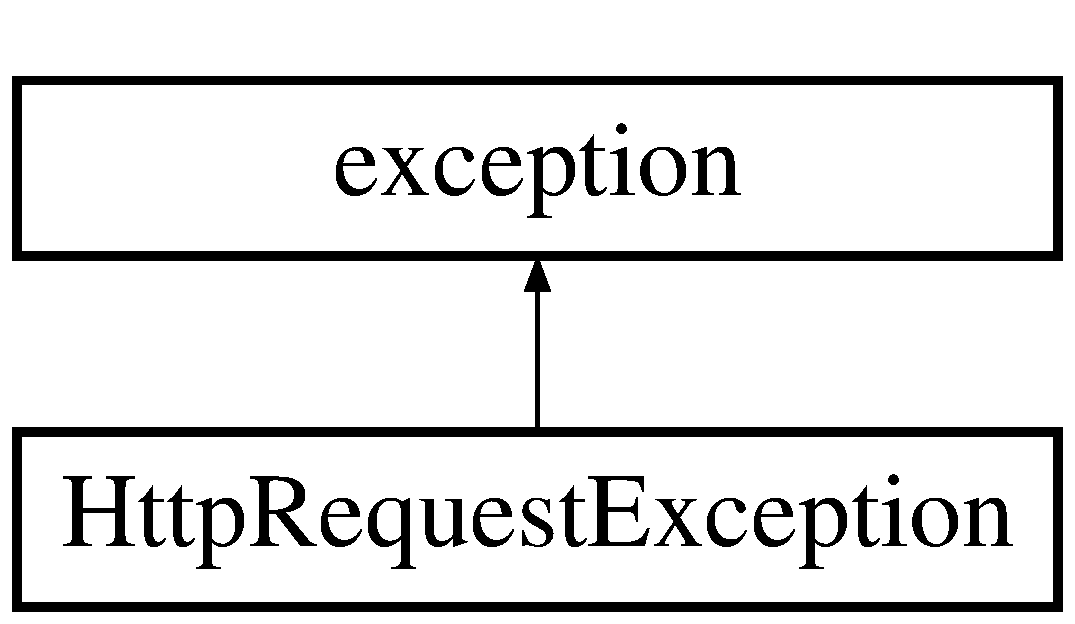
\includegraphics[height=2.000000cm]{structHttpRequestException}
\end{center}
\end{figure}
\subsection*{Public Member Functions}
\begin{DoxyCompactItemize}
\item 
\hypertarget{structHttpRequestException_a8470fe285f8e7f0939b5068546967764}{\hyperlink{structHttpRequestException_a8470fe285f8e7f0939b5068546967764}{Http\-Request\-Exception} (std\-::string msg)}\label{structHttpRequestException_a8470fe285f8e7f0939b5068546967764}

\begin{DoxyCompactList}\small\item\em Create a H\-T\-T\-P \hyperlink{structRequest}{Request} Exception, and store the given error message. \end{DoxyCompactList}\item 
\hypertarget{structHttpRequestException_acf07a2f7382157a27c0c5d2cedb2f2e6}{const char $\ast$ \hyperlink{structHttpRequestException_acf07a2f7382157a27c0c5d2cedb2f2e6}{what} () const   throw ()}\label{structHttpRequestException_acf07a2f7382157a27c0c5d2cedb2f2e6}

\begin{DoxyCompactList}\small\item\em Show the error message in readable format. \end{DoxyCompactList}\end{DoxyCompactItemize}
\subsection*{Public Attributes}
\begin{DoxyCompactItemize}
\item 
\hypertarget{structHttpRequestException_a52a64d4648b543b81050bec3fb039e5f}{std\-::string \hyperlink{structHttpRequestException_a52a64d4648b543b81050bec3fb039e5f}{int\-\_\-msg}}\label{structHttpRequestException_a52a64d4648b543b81050bec3fb039e5f}

\begin{DoxyCompactList}\small\item\em An error message passed on initialization. \end{DoxyCompactList}\end{DoxyCompactItemize}


\subsection{Detailed Description}
An Implementation of std\-::exception that denotes an error during an http operation. 

The documentation for this struct was generated from the following file\-:\begin{DoxyCompactItemize}
\item 
lib/include/factory/http\-\_\-interface.\-h\end{DoxyCompactItemize}

\hypertarget{classHttpServerInterface}{\section{Http\-Server\-Interface Class Reference}
\label{classHttpServerInterface}\index{Http\-Server\-Interface@{Http\-Server\-Interface}}
}


This is a basic H\-T\-T\-P Server that can be used to build a R\-E\-S\-Tful A\-P\-I.  




{\ttfamily \#include $<$http\-\_\-server\-\_\-interface.\-h$>$}

\subsection*{Public Member Functions}
\begin{DoxyCompactItemize}
\item 
\hypertarget{classHttpServerInterface_a6aa54efaf6f176d985c7faa57e1aa7fd}{virtual bool \hyperlink{classHttpServerInterface_a6aa54efaf6f176d985c7faa57e1aa7fd}{bind\-\_\-callback} (std\-::string uri, Callback\-Interface func)=0}\label{classHttpServerInterface_a6aa54efaf6f176d985c7faa57e1aa7fd}

\begin{DoxyCompactList}\small\item\em Bind a callback for a static A\-P\-I Method. \end{DoxyCompactList}\item 
\hypertarget{classHttpServerInterface_a398064a0d7fb0c7e52d94ccfcbb6d89a}{virtual bool \hyperlink{classHttpServerInterface_a398064a0d7fb0c7e52d94ccfcbb6d89a}{bind\-\_\-default\-\_\-callback} (Callback\-Interface func)=0}\label{classHttpServerInterface_a398064a0d7fb0c7e52d94ccfcbb6d89a}

\begin{DoxyCompactList}\small\item\em Bind a callback for a dynamic A\-P\-I Method. \end{DoxyCompactList}\item 
\hypertarget{classHttpServerInterface_a350f4321505079d9c440ce4a4372044f}{virtual void \hyperlink{classHttpServerInterface_a350f4321505079d9c440ce4a4372044f}{recv} ()=0}\label{classHttpServerInterface_a350f4321505079d9c440ce4a4372044f}

\begin{DoxyCompactList}\small\item\em Blocking call for waiting for incoming A\-P\-I Calls. \end{DoxyCompactList}\end{DoxyCompactItemize}


\subsection{Detailed Description}
This is a basic H\-T\-T\-P Server that can be used to build a R\-E\-S\-Tful A\-P\-I. 

The H\-T\-T\-P Server can bind static A\-P\-I methods to individual callbacks, and dynamic A\-P\-I methods can go to a default callback. Used to build R\-E\-S\-Tful A\-P\-I's 

The documentation for this class was generated from the following file\-:\begin{DoxyCompactItemize}
\item 
lib/include/factory/http\-\_\-server\-\_\-interface.\-h\end{DoxyCompactItemize}

\hypertarget{classInterpreter}{\section{Interpreter Class Reference}
\label{classInterpreter}\index{Interpreter@{Interpreter}}
}


\hyperlink{classInterpreter}{Interpreter} Interface.  




{\ttfamily \#include $<$interpreter.\-h$>$}

Inheritance diagram for Interpreter\-:\begin{figure}[H]
\begin{center}
\leavevmode
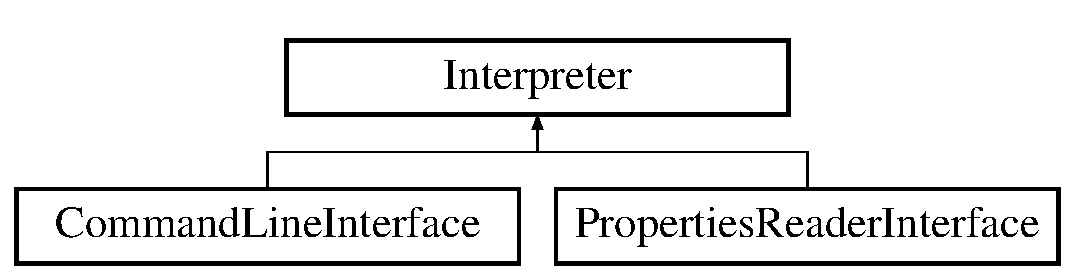
\includegraphics[height=2.000000cm]{classInterpreter}
\end{center}
\end{figure}
\subsection*{Public Member Functions}
\begin{DoxyCompactItemize}
\item 
\hypertarget{classInterpreter_a2198ba5fcff114e80fb9241f0c8960ea}{virtual bool \hyperlink{classInterpreter_a2198ba5fcff114e80fb9241f0c8960ea}{opt\-\_\-exist} (std\-::string key)=0}\label{classInterpreter_a2198ba5fcff114e80fb9241f0c8960ea}

\begin{DoxyCompactList}\small\item\em Does a key exist? \end{DoxyCompactList}\item 
\hypertarget{classInterpreter_ab315fb1a6a89b321aaadd6eb6fd6739f}{virtual std\-::string \hyperlink{classInterpreter_ab315fb1a6a89b321aaadd6eb6fd6739f}{get\-\_\-opt} (std\-::string key)=0}\label{classInterpreter_ab315fb1a6a89b321aaadd6eb6fd6739f}

\begin{DoxyCompactList}\small\item\em Get an option by key. \end{DoxyCompactList}\end{DoxyCompactItemize}


\subsection{Detailed Description}
\hyperlink{classInterpreter}{Interpreter} Interface. 

The interpreter generates a list of options that are exposed based on some input, whether it is via command line, properties file, or other methods. 

The documentation for this class was generated from the following file\-:\begin{DoxyCompactItemize}
\item 
lib/include/factory/interpreter.\-h\end{DoxyCompactItemize}

\hypertarget{classLoggingCategoryInterface}{}\section{Logging\+Category\+Interface Class Reference}
\label{classLoggingCategoryInterface}\index{Logging\+Category\+Interface@{Logging\+Category\+Interface}}


A Logging Category instantiated on a standard logging instance.  




{\ttfamily \#include $<$logging\+\_\+interface.\+h$>$}

\subsection*{Public Member Functions}
\begin{DoxyCompactItemize}
\item 
virtual void \hyperlink{classLoggingCategoryInterface_aca90c0a8380658a3918ee4c6eb60314b}{debug} (std\+::string msg)=0\hypertarget{classLoggingCategoryInterface_aca90c0a8380658a3918ee4c6eb60314b}{}\label{classLoggingCategoryInterface_aca90c0a8380658a3918ee4c6eb60314b}

\begin{DoxyCompactList}\small\item\em Log at a debug level to the root category. \end{DoxyCompactList}\item 
virtual void \hyperlink{classLoggingCategoryInterface_a377b5248cd5f1c67dc7f13250bf56d78}{error} (std\+::string msg)=0\hypertarget{classLoggingCategoryInterface_a377b5248cd5f1c67dc7f13250bf56d78}{}\label{classLoggingCategoryInterface_a377b5248cd5f1c67dc7f13250bf56d78}

\begin{DoxyCompactList}\small\item\em Log at an error level to the root category. \end{DoxyCompactList}\item 
virtual void \hyperlink{classLoggingCategoryInterface_a2a8bf026f9aeaea95f443744292e237b}{info} (std\+::string msg)=0\hypertarget{classLoggingCategoryInterface_a2a8bf026f9aeaea95f443744292e237b}{}\label{classLoggingCategoryInterface_a2a8bf026f9aeaea95f443744292e237b}

\begin{DoxyCompactList}\small\item\em Log at an info level to the root category. \end{DoxyCompactList}\item 
virtual void \hyperlink{classLoggingCategoryInterface_a6633ea62fbd9850de9f95c42bcb98209}{debug} (const char $\ast$msg)=0\hypertarget{classLoggingCategoryInterface_a6633ea62fbd9850de9f95c42bcb98209}{}\label{classLoggingCategoryInterface_a6633ea62fbd9850de9f95c42bcb98209}

\begin{DoxyCompactList}\small\item\em Log at an debug level to the root category. \end{DoxyCompactList}\item 
virtual void \hyperlink{classLoggingCategoryInterface_a526c3bec470411e17b10a6f38b5477c6}{error} (const char $\ast$msg)=0\hypertarget{classLoggingCategoryInterface_a526c3bec470411e17b10a6f38b5477c6}{}\label{classLoggingCategoryInterface_a526c3bec470411e17b10a6f38b5477c6}

\begin{DoxyCompactList}\small\item\em Log at an error level to the root category. \end{DoxyCompactList}\item 
virtual void \hyperlink{classLoggingCategoryInterface_a5e05b670e8298e0016af09ee5d1c50a6}{info} (const char $\ast$msg)=0\hypertarget{classLoggingCategoryInterface_a5e05b670e8298e0016af09ee5d1c50a6}{}\label{classLoggingCategoryInterface_a5e05b670e8298e0016af09ee5d1c50a6}

\begin{DoxyCompactList}\small\item\em Log at an info level to the root category. \end{DoxyCompactList}\item 
virtual void \hyperlink{classLoggingCategoryInterface_a29536210dbd4617a058cfdad8f8da850}{debug} (int msg)=0\hypertarget{classLoggingCategoryInterface_a29536210dbd4617a058cfdad8f8da850}{}\label{classLoggingCategoryInterface_a29536210dbd4617a058cfdad8f8da850}

\begin{DoxyCompactList}\small\item\em Log at an debug level to the root category. \end{DoxyCompactList}\item 
virtual void \hyperlink{classLoggingCategoryInterface_a5dca5bda32f0f504f2ff2e8a6706f64f}{error} (int msg)=0\hypertarget{classLoggingCategoryInterface_a5dca5bda32f0f504f2ff2e8a6706f64f}{}\label{classLoggingCategoryInterface_a5dca5bda32f0f504f2ff2e8a6706f64f}

\begin{DoxyCompactList}\small\item\em Log at an error level to the root category. \end{DoxyCompactList}\item 
virtual void \hyperlink{classLoggingCategoryInterface_a2c7085aa124ef1e055b43a3c1f4aa866}{info} (int msg)=0\hypertarget{classLoggingCategoryInterface_a2c7085aa124ef1e055b43a3c1f4aa866}{}\label{classLoggingCategoryInterface_a2c7085aa124ef1e055b43a3c1f4aa866}

\begin{DoxyCompactList}\small\item\em Log at an info level to the root category. \end{DoxyCompactList}\item 
virtual void \hyperlink{classLoggingCategoryInterface_aef995a06be8f48121250ceb545ee9ce8}{debug} (float msg)=0\hypertarget{classLoggingCategoryInterface_aef995a06be8f48121250ceb545ee9ce8}{}\label{classLoggingCategoryInterface_aef995a06be8f48121250ceb545ee9ce8}

\begin{DoxyCompactList}\small\item\em Log at an debug level to the root category. \end{DoxyCompactList}\item 
virtual void \hyperlink{classLoggingCategoryInterface_a288016acac317ac5feb149506650431b}{error} (float msg)=0\hypertarget{classLoggingCategoryInterface_a288016acac317ac5feb149506650431b}{}\label{classLoggingCategoryInterface_a288016acac317ac5feb149506650431b}

\begin{DoxyCompactList}\small\item\em Log at an error level to the root category. \end{DoxyCompactList}\item 
virtual void \hyperlink{classLoggingCategoryInterface_abc7a15e2c8befa164be1a0a98df8de26}{info} (float msg)=0\hypertarget{classLoggingCategoryInterface_abc7a15e2c8befa164be1a0a98df8de26}{}\label{classLoggingCategoryInterface_abc7a15e2c8befa164be1a0a98df8de26}

\begin{DoxyCompactList}\small\item\em Log at an info level to the root category. \end{DoxyCompactList}\item 
virtual void \hyperlink{classLoggingCategoryInterface_a12ee058f0418ff5bee7b598df79be600}{debug} (double msg)=0\hypertarget{classLoggingCategoryInterface_a12ee058f0418ff5bee7b598df79be600}{}\label{classLoggingCategoryInterface_a12ee058f0418ff5bee7b598df79be600}

\begin{DoxyCompactList}\small\item\em Log at an debug level to the root category. \end{DoxyCompactList}\item 
virtual void \hyperlink{classLoggingCategoryInterface_a157483fef60e45eb2f6f0d7698d11880}{error} (double msg)=0\hypertarget{classLoggingCategoryInterface_a157483fef60e45eb2f6f0d7698d11880}{}\label{classLoggingCategoryInterface_a157483fef60e45eb2f6f0d7698d11880}

\begin{DoxyCompactList}\small\item\em Log at an error level to the root category. \end{DoxyCompactList}\item 
virtual void \hyperlink{classLoggingCategoryInterface_aa99020d66ab28b686e060112b395b49f}{info} (double msg)=0\hypertarget{classLoggingCategoryInterface_aa99020d66ab28b686e060112b395b49f}{}\label{classLoggingCategoryInterface_aa99020d66ab28b686e060112b395b49f}

\begin{DoxyCompactList}\small\item\em Log at an info level to the root category. \end{DoxyCompactList}\end{DoxyCompactItemize}


\subsection{Detailed Description}
A Logging Category instantiated on a standard logging instance. 

The documentation for this class was generated from the following file\+:\begin{DoxyCompactItemize}
\item 
aossl/logging/include/logging\+\_\+interface.\+h\end{DoxyCompactItemize}

\hypertarget{classLoggingInterface}{}\section{Logging\+Interface Class Reference}
\label{classLoggingInterface}\index{Logging\+Interface@{Logging\+Interface}}


An overall logging interface, which can generate logging categories.  




{\ttfamily \#include $<$logging\+\_\+interface.\+h$>$}

\subsection*{Public Member Functions}
\begin{DoxyCompactItemize}
\item 
virtual void \hyperlink{classLoggingInterface_a94e666bf17b42a65c03aff86cbe04978}{debug} (std\+::string msg)=0\hypertarget{classLoggingInterface_a94e666bf17b42a65c03aff86cbe04978}{}\label{classLoggingInterface_a94e666bf17b42a65c03aff86cbe04978}

\begin{DoxyCompactList}\small\item\em Log at a debug level to the root category. \end{DoxyCompactList}\item 
virtual void \hyperlink{classLoggingInterface_a86ba6616c2163d8cb49bed70def8b862}{error} (std\+::string msg)=0\hypertarget{classLoggingInterface_a86ba6616c2163d8cb49bed70def8b862}{}\label{classLoggingInterface_a86ba6616c2163d8cb49bed70def8b862}

\begin{DoxyCompactList}\small\item\em Log at an error level to the root category. \end{DoxyCompactList}\item 
virtual void \hyperlink{classLoggingInterface_a5d994f7cfafe81171954409df64d77ce}{info} (std\+::string msg)=0\hypertarget{classLoggingInterface_a5d994f7cfafe81171954409df64d77ce}{}\label{classLoggingInterface_a5d994f7cfafe81171954409df64d77ce}

\begin{DoxyCompactList}\small\item\em Log at an info level to the root category. \end{DoxyCompactList}\item 
virtual void \hyperlink{classLoggingInterface_a82c2727fb66531d5eec19e39bed79671}{debug} (const char $\ast$msg)=0\hypertarget{classLoggingInterface_a82c2727fb66531d5eec19e39bed79671}{}\label{classLoggingInterface_a82c2727fb66531d5eec19e39bed79671}

\begin{DoxyCompactList}\small\item\em Log at an debug level to the root category. \end{DoxyCompactList}\item 
virtual void \hyperlink{classLoggingInterface_a1cea9e37dae316f39e171654e5e0dc0f}{error} (const char $\ast$msg)=0\hypertarget{classLoggingInterface_a1cea9e37dae316f39e171654e5e0dc0f}{}\label{classLoggingInterface_a1cea9e37dae316f39e171654e5e0dc0f}

\begin{DoxyCompactList}\small\item\em Log at an error level to the root category. \end{DoxyCompactList}\item 
virtual void \hyperlink{classLoggingInterface_a7aed25910dd1cdebe3906b4b33d75a80}{info} (const char $\ast$msg)=0\hypertarget{classLoggingInterface_a7aed25910dd1cdebe3906b4b33d75a80}{}\label{classLoggingInterface_a7aed25910dd1cdebe3906b4b33d75a80}

\begin{DoxyCompactList}\small\item\em Log at an info level to the root category. \end{DoxyCompactList}\item 
virtual void \hyperlink{classLoggingInterface_a66b4e3f845501917df8975e95157f436}{debug} (int msg)=0\hypertarget{classLoggingInterface_a66b4e3f845501917df8975e95157f436}{}\label{classLoggingInterface_a66b4e3f845501917df8975e95157f436}

\begin{DoxyCompactList}\small\item\em Log at an debug level to the root category. \end{DoxyCompactList}\item 
virtual void \hyperlink{classLoggingInterface_a85fa61f75508d25d846f7ac39790c457}{error} (int msg)=0\hypertarget{classLoggingInterface_a85fa61f75508d25d846f7ac39790c457}{}\label{classLoggingInterface_a85fa61f75508d25d846f7ac39790c457}

\begin{DoxyCompactList}\small\item\em Log at an error level to the root category. \end{DoxyCompactList}\item 
virtual void \hyperlink{classLoggingInterface_a724cb769b7233a783956e9fa41ff7291}{info} (int msg)=0\hypertarget{classLoggingInterface_a724cb769b7233a783956e9fa41ff7291}{}\label{classLoggingInterface_a724cb769b7233a783956e9fa41ff7291}

\begin{DoxyCompactList}\small\item\em Log at an info level to the root category. \end{DoxyCompactList}\item 
virtual void \hyperlink{classLoggingInterface_a301a0e53971f7fabd6f296722738aeff}{debug} (float msg)=0\hypertarget{classLoggingInterface_a301a0e53971f7fabd6f296722738aeff}{}\label{classLoggingInterface_a301a0e53971f7fabd6f296722738aeff}

\begin{DoxyCompactList}\small\item\em Log at an debug level to the root category. \end{DoxyCompactList}\item 
virtual void \hyperlink{classLoggingInterface_adab4f9849012eca577d04981e185d08c}{error} (float msg)=0\hypertarget{classLoggingInterface_adab4f9849012eca577d04981e185d08c}{}\label{classLoggingInterface_adab4f9849012eca577d04981e185d08c}

\begin{DoxyCompactList}\small\item\em Log at an error level to the root category. \end{DoxyCompactList}\item 
virtual void \hyperlink{classLoggingInterface_aebe8b51717ca65efb39cea955aa24e73}{info} (float msg)=0\hypertarget{classLoggingInterface_aebe8b51717ca65efb39cea955aa24e73}{}\label{classLoggingInterface_aebe8b51717ca65efb39cea955aa24e73}

\begin{DoxyCompactList}\small\item\em Log at an info level to the root category. \end{DoxyCompactList}\item 
virtual void \hyperlink{classLoggingInterface_afbb073b280b346f52b1b26be9aad9c9c}{debug} (double msg)=0\hypertarget{classLoggingInterface_afbb073b280b346f52b1b26be9aad9c9c}{}\label{classLoggingInterface_afbb073b280b346f52b1b26be9aad9c9c}

\begin{DoxyCompactList}\small\item\em Log at an debug level to the root category. \end{DoxyCompactList}\item 
virtual void \hyperlink{classLoggingInterface_ad7e7ef57f8aba34cb9df9788b52faae7}{error} (double msg)=0\hypertarget{classLoggingInterface_ad7e7ef57f8aba34cb9df9788b52faae7}{}\label{classLoggingInterface_ad7e7ef57f8aba34cb9df9788b52faae7}

\begin{DoxyCompactList}\small\item\em Log at an error level to the root category. \end{DoxyCompactList}\item 
virtual void \hyperlink{classLoggingInterface_a6e196d311e2b078071a3a4a8337a6264}{info} (double msg)=0\hypertarget{classLoggingInterface_a6e196d311e2b078071a3a4a8337a6264}{}\label{classLoggingInterface_a6e196d311e2b078071a3a4a8337a6264}

\begin{DoxyCompactList}\small\item\em Log at an info level to the root category. \end{DoxyCompactList}\item 
virtual \hyperlink{classLoggingCategoryInterface}{Logging\+Category\+Interface} $\ast$ \hyperlink{classLoggingInterface_add380ece858220c46aeb38ce1531a6c7}{get\+\_\+category} (std\+::string name)=0\hypertarget{classLoggingInterface_add380ece858220c46aeb38ce1531a6c7}{}\label{classLoggingInterface_add380ece858220c46aeb38ce1531a6c7}

\begin{DoxyCompactList}\small\item\em Pull down different categories by name. \end{DoxyCompactList}\end{DoxyCompactItemize}


\subsection{Detailed Description}
An overall logging interface, which can generate logging categories. 

The documentation for this class was generated from the following file\+:\begin{DoxyCompactItemize}
\item 
aossl/logging/include/logging\+\_\+interface.\+h\end{DoxyCompactItemize}

\hypertarget{structMongoException}{\section{Mongo\-Exception Struct Reference}
\label{structMongoException}\index{Mongo\-Exception@{Mongo\-Exception}}
}
Inheritance diagram for Mongo\-Exception\-:\begin{figure}[H]
\begin{center}
\leavevmode
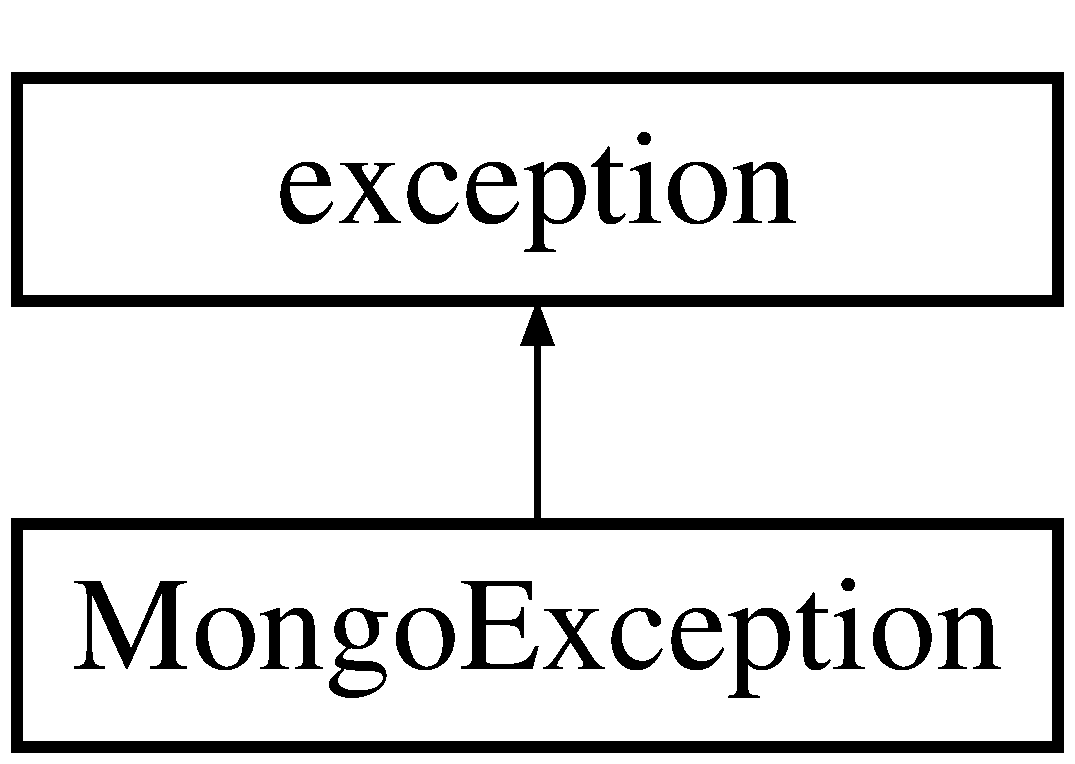
\includegraphics[height=2.000000cm]{structMongoException}
\end{center}
\end{figure}
\subsection*{Public Member Functions}
\begin{DoxyCompactItemize}
\item 
\hypertarget{structMongoException_addaa545189ab30bcc6a0e957514253fa}{\hyperlink{structMongoException_addaa545189ab30bcc6a0e957514253fa}{Mongo\-Exception} (std\-::string msg)}\label{structMongoException_addaa545189ab30bcc6a0e957514253fa}

\begin{DoxyCompactList}\small\item\em Create a Mongo Exception, and store the given error message. \end{DoxyCompactList}\item 
\hypertarget{structMongoException_a5202b0dfc3d8a554d9f36e4b1c31c2a3}{const char $\ast$ \hyperlink{structMongoException_a5202b0dfc3d8a554d9f36e4b1c31c2a3}{what} () const   throw ()}\label{structMongoException_a5202b0dfc3d8a554d9f36e4b1c31c2a3}

\begin{DoxyCompactList}\small\item\em Show the error message in readable format. \end{DoxyCompactList}\end{DoxyCompactItemize}
\subsection*{Public Attributes}
\begin{DoxyCompactItemize}
\item 
\hypertarget{structMongoException_ae5a0824b7a469b66dcc3947704310e4c}{std\-::string \hyperlink{structMongoException_ae5a0824b7a469b66dcc3947704310e4c}{int\-\_\-msg}}\label{structMongoException_ae5a0824b7a469b66dcc3947704310e4c}

\begin{DoxyCompactList}\small\item\em An error message passed on initialization. \end{DoxyCompactList}\end{DoxyCompactItemize}


The documentation for this struct was generated from the following file\-:\begin{DoxyCompactItemize}
\item 
lib/include/factory/mongo\-\_\-interface.\-h\end{DoxyCompactItemize}

\hypertarget{classMongoInterface}{}\section{Mongo\+Interface Class Reference}
\label{classMongoInterface}\index{Mongo\+Interface@{Mongo\+Interface}}
\subsection*{Public Member Functions}
\begin{DoxyCompactItemize}
\item 
virtual \hyperlink{classMongoResponseInterface}{Mongo\+Response\+Interface} $\ast$ \hyperlink{classMongoInterface_a40a5973d65dd15c46df9f6c06fbb464a}{create\+\_\+document} (const char $\ast$doc, const char $\ast$collection\+\_\+name)=0\hypertarget{classMongoInterface_a40a5973d65dd15c46df9f6c06fbb464a}{}\label{classMongoInterface_a40a5973d65dd15c46df9f6c06fbb464a}

\begin{DoxyCompactList}\small\item\em Create J\+S\+ON Document, returns the document key. \end{DoxyCompactList}\item 
virtual \hyperlink{classMongoResponseInterface}{Mongo\+Response\+Interface} $\ast$ \hyperlink{classMongoInterface_af621e8af8a4205e1cf06d1964ba36843}{create\+\_\+document} (const char $\ast$doc)=0\hypertarget{classMongoInterface_af621e8af8a4205e1cf06d1964ba36843}{}\label{classMongoInterface_af621e8af8a4205e1cf06d1964ba36843}

\begin{DoxyCompactList}\small\item\em Create J\+S\+ON Document, returns the document key. \end{DoxyCompactList}\item 
virtual \hyperlink{classMongoResponseInterface}{Mongo\+Response\+Interface} $\ast$ \hyperlink{classMongoInterface_aaa549157c25eef7e9ed21b143c28bb64}{create\+\_\+document} (std\+::string doc)=0\hypertarget{classMongoInterface_aaa549157c25eef7e9ed21b143c28bb64}{}\label{classMongoInterface_aaa549157c25eef7e9ed21b143c28bb64}

\begin{DoxyCompactList}\small\item\em Create J\+S\+ON Document, returns the document key. \end{DoxyCompactList}\item 
virtual \hyperlink{classMongoResponseInterface}{Mongo\+Response\+Interface} $\ast$ \hyperlink{classMongoInterface_a5870d9a0cb64044d195893cc4d59801f}{create\+\_\+document} (std\+::string doc, std\+::string collection\+\_\+name)=0\hypertarget{classMongoInterface_a5870d9a0cb64044d195893cc4d59801f}{}\label{classMongoInterface_a5870d9a0cb64044d195893cc4d59801f}

\begin{DoxyCompactList}\small\item\em Create J\+S\+ON Document, returns the document key. \end{DoxyCompactList}\item 
virtual void \hyperlink{classMongoInterface_a9153c6d0c292aa76e51bf65c41d51f8d}{delete\+\_\+document} (const char $\ast$key)=0\hypertarget{classMongoInterface_a9153c6d0c292aa76e51bf65c41d51f8d}{}\label{classMongoInterface_a9153c6d0c292aa76e51bf65c41d51f8d}

\begin{DoxyCompactList}\small\item\em Delete a J\+S\+ON Document, returns true if successful. \end{DoxyCompactList}\item 
virtual void \hyperlink{classMongoInterface_a9e15069c0c05f9aa89918fd39c0e7a94}{delete\+\_\+document} (std\+::string key)=0\hypertarget{classMongoInterface_a9e15069c0c05f9aa89918fd39c0e7a94}{}\label{classMongoInterface_a9e15069c0c05f9aa89918fd39c0e7a94}

\begin{DoxyCompactList}\small\item\em Delete a J\+S\+ON Document, returns true if successful. \end{DoxyCompactList}\item 
virtual void \hyperlink{classMongoInterface_abc9fd636d41e508ede790754e4dbab86}{delete\+\_\+document} (const char $\ast$key, const char $\ast$collection\+\_\+name)=0\hypertarget{classMongoInterface_abc9fd636d41e508ede790754e4dbab86}{}\label{classMongoInterface_abc9fd636d41e508ede790754e4dbab86}

\begin{DoxyCompactList}\small\item\em Delete a J\+S\+ON Document, returns true if successful. \end{DoxyCompactList}\item 
virtual void \hyperlink{classMongoInterface_ae00271d50df56c537627031c0ecef0d6}{delete\+\_\+document} (std\+::string key, std\+::string collection\+\_\+name)=0\hypertarget{classMongoInterface_ae00271d50df56c537627031c0ecef0d6}{}\label{classMongoInterface_ae00271d50df56c537627031c0ecef0d6}

\begin{DoxyCompactList}\small\item\em Delete a J\+S\+ON Document, returns true if successful. \end{DoxyCompactList}\item 
virtual \hyperlink{classMongoResponseInterface}{Mongo\+Response\+Interface} $\ast$ \hyperlink{classMongoInterface_acc6a2b3cc3cf9dcbc0cdb44ddbd14674}{load\+\_\+document} (const char $\ast$key)=0\hypertarget{classMongoInterface_acc6a2b3cc3cf9dcbc0cdb44ddbd14674}{}\label{classMongoInterface_acc6a2b3cc3cf9dcbc0cdb44ddbd14674}

\begin{DoxyCompactList}\small\item\em Retrieve a J\+S\+ON Document and return it in a std\+::string. \end{DoxyCompactList}\item 
virtual \hyperlink{classMongoResponseInterface}{Mongo\+Response\+Interface} $\ast$ \hyperlink{classMongoInterface_a19e569ead19f32799fa49805a6345551}{load\+\_\+document} (std\+::string key)=0\hypertarget{classMongoInterface_a19e569ead19f32799fa49805a6345551}{}\label{classMongoInterface_a19e569ead19f32799fa49805a6345551}

\begin{DoxyCompactList}\small\item\em Retrieve a J\+S\+ON Document and return it in a std\+::string. \end{DoxyCompactList}\item 
virtual \hyperlink{classMongoResponseInterface}{Mongo\+Response\+Interface} $\ast$ \hyperlink{classMongoInterface_abb8bf5ca5eed49b76fd91adcf3a8dfc8}{load\+\_\+document} (const char $\ast$key, const char $\ast$collection\+\_\+name)=0\hypertarget{classMongoInterface_abb8bf5ca5eed49b76fd91adcf3a8dfc8}{}\label{classMongoInterface_abb8bf5ca5eed49b76fd91adcf3a8dfc8}

\begin{DoxyCompactList}\small\item\em Retrieve a J\+S\+ON Document and return it in a std\+::string. \end{DoxyCompactList}\item 
virtual \hyperlink{classMongoResponseInterface}{Mongo\+Response\+Interface} $\ast$ \hyperlink{classMongoInterface_a7635ac63b0968306687632d037df5d4a}{load\+\_\+document} (std\+::string key, std\+::string collection\+\_\+name)=0\hypertarget{classMongoInterface_a7635ac63b0968306687632d037df5d4a}{}\label{classMongoInterface_a7635ac63b0968306687632d037df5d4a}

\begin{DoxyCompactList}\small\item\em Retrieve a J\+S\+ON Document and return it in a std\+::string. \end{DoxyCompactList}\item 
virtual void \hyperlink{classMongoInterface_a05885b7361096a03b623da8c7b48e461}{save\+\_\+document} (const char $\ast$doc, const char $\ast$key)=0\hypertarget{classMongoInterface_a05885b7361096a03b623da8c7b48e461}{}\label{classMongoInterface_a05885b7361096a03b623da8c7b48e461}

\begin{DoxyCompactList}\small\item\em Update an existing document, returns true if successful. \end{DoxyCompactList}\item 
virtual void \hyperlink{classMongoInterface_a35888cb594d1f46d52147649786e948f}{save\+\_\+document} (std\+::string doc, std\+::string key)=0\hypertarget{classMongoInterface_a35888cb594d1f46d52147649786e948f}{}\label{classMongoInterface_a35888cb594d1f46d52147649786e948f}

\begin{DoxyCompactList}\small\item\em Update an existing document, returns true if successful. \end{DoxyCompactList}\item 
virtual void \hyperlink{classMongoInterface_a4d2c3e6a8fb172f8d07fc3dd710053ae}{save\+\_\+document} (const char $\ast$doc, const char $\ast$key, const char $\ast$collection\+\_\+name)=0\hypertarget{classMongoInterface_a4d2c3e6a8fb172f8d07fc3dd710053ae}{}\label{classMongoInterface_a4d2c3e6a8fb172f8d07fc3dd710053ae}

\begin{DoxyCompactList}\small\item\em Update an existing document, returns true if successful. \end{DoxyCompactList}\item 
virtual void \hyperlink{classMongoInterface_a14f3c2a76a495777a1f48ed155831134}{save\+\_\+document} (std\+::string doc, std\+::string key, std\+::string collection\+\_\+name)=0\hypertarget{classMongoInterface_a14f3c2a76a495777a1f48ed155831134}{}\label{classMongoInterface_a14f3c2a76a495777a1f48ed155831134}

\begin{DoxyCompactList}\small\item\em Update an existing document, returns true if successful. \end{DoxyCompactList}\item 
virtual \hyperlink{classMongoIteratorInterface}{Mongo\+Iterator\+Interface} $\ast$ \hyperlink{classMongoInterface_a15ceb9bc80b43bc09afd0d5e32cea4f7}{query} (const char $\ast$query\+\_\+str, const char $\ast$opts\+\_\+str)=0
\begin{DoxyCompactList}\small\item\em Queries. \end{DoxyCompactList}\item 
virtual \hyperlink{classMongoIteratorInterface}{Mongo\+Iterator\+Interface} $\ast$ \hyperlink{classMongoInterface_a6f5d8758fe477e997df995028afe82a4}{query} (std\+::string query\+\_\+str, std\+::string opts\+\_\+str)=0
\begin{DoxyCompactList}\small\item\em Queries. \end{DoxyCompactList}\item 
virtual \hyperlink{classMongoIteratorInterface}{Mongo\+Iterator\+Interface} $\ast$ \hyperlink{classMongoInterface_ab4aa9b1a60d96ffcf787114fc2d436b0}{query} (const char $\ast$query\+\_\+str, const char $\ast$opts\+\_\+str, const char $\ast$collection\+\_\+name)=0
\begin{DoxyCompactList}\small\item\em Queries. \end{DoxyCompactList}\item 
virtual \hyperlink{classMongoIteratorInterface}{Mongo\+Iterator\+Interface} $\ast$ \hyperlink{classMongoInterface_a37fd750f45fc0a9b7360c3ad433c1747}{query} (std\+::string query\+\_\+str, std\+::string opts\+\_\+str, std\+::string collection\+\_\+name)=0
\begin{DoxyCompactList}\small\item\em Queries. \end{DoxyCompactList}\item 
virtual \hyperlink{classMongoIteratorInterface}{Mongo\+Iterator\+Interface} $\ast$ \hyperlink{classMongoInterface_a53f62c62e8a54abcb6ead11e544b51d0}{query} (const char $\ast$query\+\_\+str)=0
\begin{DoxyCompactList}\small\item\em Queries. \end{DoxyCompactList}\item 
virtual \hyperlink{classMongoIteratorInterface}{Mongo\+Iterator\+Interface} $\ast$ \hyperlink{classMongoInterface_afbfd334e99d9c1861ea9c4623b326e48}{query} (std\+::string query\+\_\+str)=0
\begin{DoxyCompactList}\small\item\em Queries. \end{DoxyCompactList}\end{DoxyCompactItemize}


\subsection{Member Function Documentation}
\index{Mongo\+Interface@{Mongo\+Interface}!query@{query}}
\index{query@{query}!Mongo\+Interface@{Mongo\+Interface}}
\subsubsection[{\texorpdfstring{query(const char $\ast$query\+\_\+str, const char $\ast$opts\+\_\+str)=0}{query(const char *query_str, const char *opts_str)=0}}]{\setlength{\rightskip}{0pt plus 5cm}virtual {\bf Mongo\+Iterator\+Interface}$\ast$ Mongo\+Interface\+::query (
\begin{DoxyParamCaption}
\item[{const char $\ast$}]{query\+\_\+str, }
\item[{const char $\ast$}]{opts\+\_\+str}
\end{DoxyParamCaption}
)\hspace{0.3cm}{\ttfamily [pure virtual]}}\hypertarget{classMongoInterface_a15ceb9bc80b43bc09afd0d5e32cea4f7}{}\label{classMongoInterface_a15ceb9bc80b43bc09afd0d5e32cea4f7}


Queries. 

Accept the query and query options in J\+S\+ON format. Return an iterator which can be used to access query results \index{Mongo\+Interface@{Mongo\+Interface}!query@{query}}
\index{query@{query}!Mongo\+Interface@{Mongo\+Interface}}
\subsubsection[{\texorpdfstring{query(std\+::string query\+\_\+str, std\+::string opts\+\_\+str)=0}{query(std::string query_str, std::string opts_str)=0}}]{\setlength{\rightskip}{0pt plus 5cm}virtual {\bf Mongo\+Iterator\+Interface}$\ast$ Mongo\+Interface\+::query (
\begin{DoxyParamCaption}
\item[{std\+::string}]{query\+\_\+str, }
\item[{std\+::string}]{opts\+\_\+str}
\end{DoxyParamCaption}
)\hspace{0.3cm}{\ttfamily [pure virtual]}}\hypertarget{classMongoInterface_a6f5d8758fe477e997df995028afe82a4}{}\label{classMongoInterface_a6f5d8758fe477e997df995028afe82a4}


Queries. 

Accept the query and query options in J\+S\+ON format. Return an iterator which can be used to access query results \index{Mongo\+Interface@{Mongo\+Interface}!query@{query}}
\index{query@{query}!Mongo\+Interface@{Mongo\+Interface}}
\subsubsection[{\texorpdfstring{query(const char $\ast$query\+\_\+str, const char $\ast$opts\+\_\+str, const char $\ast$collection\+\_\+name)=0}{query(const char *query_str, const char *opts_str, const char *collection_name)=0}}]{\setlength{\rightskip}{0pt plus 5cm}virtual {\bf Mongo\+Iterator\+Interface}$\ast$ Mongo\+Interface\+::query (
\begin{DoxyParamCaption}
\item[{const char $\ast$}]{query\+\_\+str, }
\item[{const char $\ast$}]{opts\+\_\+str, }
\item[{const char $\ast$}]{collection\+\_\+name}
\end{DoxyParamCaption}
)\hspace{0.3cm}{\ttfamily [pure virtual]}}\hypertarget{classMongoInterface_ab4aa9b1a60d96ffcf787114fc2d436b0}{}\label{classMongoInterface_ab4aa9b1a60d96ffcf787114fc2d436b0}


Queries. 

Accept the query and query options in J\+S\+ON format. Return an iterator which can be used to access query results \index{Mongo\+Interface@{Mongo\+Interface}!query@{query}}
\index{query@{query}!Mongo\+Interface@{Mongo\+Interface}}
\subsubsection[{\texorpdfstring{query(std\+::string query\+\_\+str, std\+::string opts\+\_\+str, std\+::string collection\+\_\+name)=0}{query(std::string query_str, std::string opts_str, std::string collection_name)=0}}]{\setlength{\rightskip}{0pt plus 5cm}virtual {\bf Mongo\+Iterator\+Interface}$\ast$ Mongo\+Interface\+::query (
\begin{DoxyParamCaption}
\item[{std\+::string}]{query\+\_\+str, }
\item[{std\+::string}]{opts\+\_\+str, }
\item[{std\+::string}]{collection\+\_\+name}
\end{DoxyParamCaption}
)\hspace{0.3cm}{\ttfamily [pure virtual]}}\hypertarget{classMongoInterface_a37fd750f45fc0a9b7360c3ad433c1747}{}\label{classMongoInterface_a37fd750f45fc0a9b7360c3ad433c1747}


Queries. 

Accept the query and query options in J\+S\+ON format. Return an iterator which can be used to access query results \index{Mongo\+Interface@{Mongo\+Interface}!query@{query}}
\index{query@{query}!Mongo\+Interface@{Mongo\+Interface}}
\subsubsection[{\texorpdfstring{query(const char $\ast$query\+\_\+str)=0}{query(const char *query_str)=0}}]{\setlength{\rightskip}{0pt plus 5cm}virtual {\bf Mongo\+Iterator\+Interface}$\ast$ Mongo\+Interface\+::query (
\begin{DoxyParamCaption}
\item[{const char $\ast$}]{query\+\_\+str}
\end{DoxyParamCaption}
)\hspace{0.3cm}{\ttfamily [pure virtual]}}\hypertarget{classMongoInterface_a53f62c62e8a54abcb6ead11e544b51d0}{}\label{classMongoInterface_a53f62c62e8a54abcb6ead11e544b51d0}


Queries. 

Accept the query in J\+S\+ON format. Return an iterator which can be used to access query results \index{Mongo\+Interface@{Mongo\+Interface}!query@{query}}
\index{query@{query}!Mongo\+Interface@{Mongo\+Interface}}
\subsubsection[{\texorpdfstring{query(std\+::string query\+\_\+str)=0}{query(std::string query_str)=0}}]{\setlength{\rightskip}{0pt plus 5cm}virtual {\bf Mongo\+Iterator\+Interface}$\ast$ Mongo\+Interface\+::query (
\begin{DoxyParamCaption}
\item[{std\+::string}]{query\+\_\+str}
\end{DoxyParamCaption}
)\hspace{0.3cm}{\ttfamily [pure virtual]}}\hypertarget{classMongoInterface_afbfd334e99d9c1861ea9c4623b326e48}{}\label{classMongoInterface_afbfd334e99d9c1861ea9c4623b326e48}


Queries. 

Accept the query in J\+S\+ON format. Return an iterator which can be used to access query results 

The documentation for this class was generated from the following file\+:\begin{DoxyCompactItemize}
\item 
aossl/mongo/include/mongo\+\_\+interface.\+h\end{DoxyCompactItemize}

\hypertarget{structNeo4jException}{\section{Neo4j\-Exception Struct Reference}
\label{structNeo4jException}\index{Neo4j\-Exception@{Neo4j\-Exception}}
}


A Neo4j Exception.  




{\ttfamily \#include $<$neo4j\-\_\-interface.\-h$>$}

Inheritance diagram for Neo4j\-Exception\-:\begin{figure}[H]
\begin{center}
\leavevmode
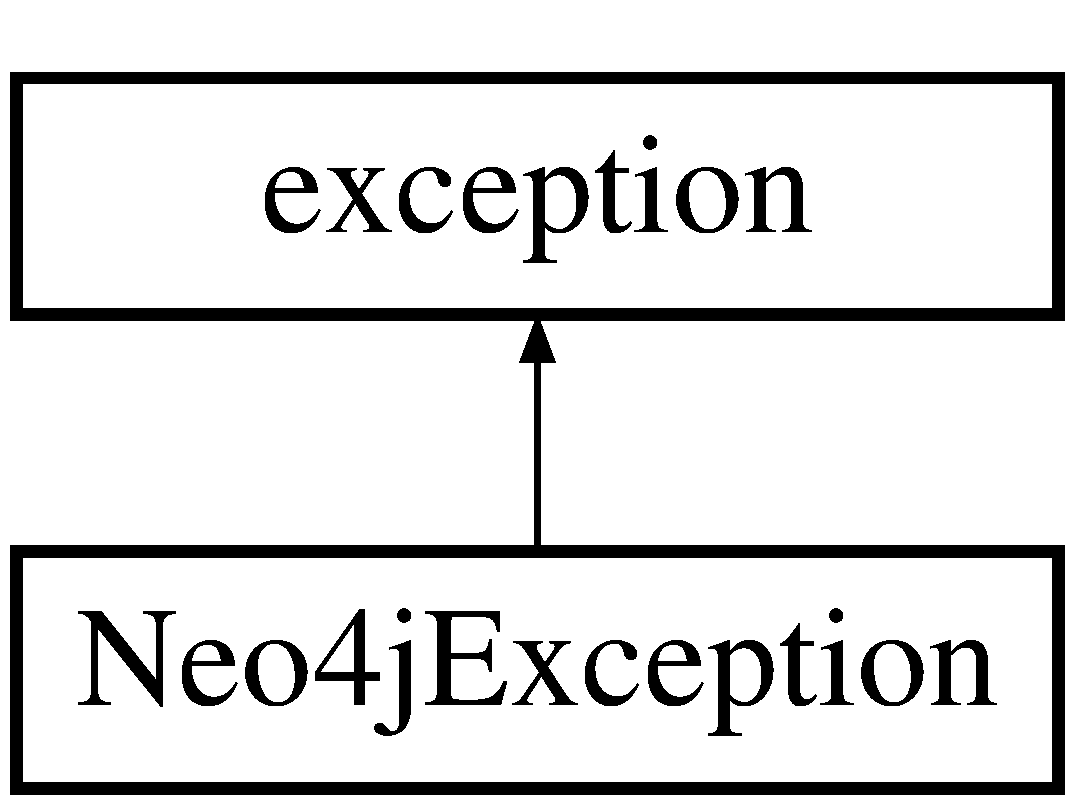
\includegraphics[height=2.000000cm]{structNeo4jException}
\end{center}
\end{figure}
\subsection*{Public Member Functions}
\begin{DoxyCompactItemize}
\item 
\hypertarget{structNeo4jException_abc88c2de520842b99f79a8df4ce04d59}{\hyperlink{structNeo4jException_abc88c2de520842b99f79a8df4ce04d59}{Neo4j\-Exception} (std\-::string msg)}\label{structNeo4jException_abc88c2de520842b99f79a8df4ce04d59}

\begin{DoxyCompactList}\small\item\em Create a Neo4j Exception, and store the given error message. \end{DoxyCompactList}\item 
\hypertarget{structNeo4jException_a2a366af8251f2aa869e64326f96e108d}{const char $\ast$ \hyperlink{structNeo4jException_a2a366af8251f2aa869e64326f96e108d}{what} () const   throw ()}\label{structNeo4jException_a2a366af8251f2aa869e64326f96e108d}

\begin{DoxyCompactList}\small\item\em Show the error message in readable format. \end{DoxyCompactList}\end{DoxyCompactItemize}
\subsection*{Public Attributes}
\begin{DoxyCompactItemize}
\item 
\hypertarget{structNeo4jException_a49252646cf779b582d6224c46586416b}{std\-::string \hyperlink{structNeo4jException_a49252646cf779b582d6224c46586416b}{int\-\_\-msg}}\label{structNeo4jException_a49252646cf779b582d6224c46586416b}

\begin{DoxyCompactList}\small\item\em An error message passed on initialization. \end{DoxyCompactList}\end{DoxyCompactItemize}


\subsection{Detailed Description}
A Neo4j Exception. 

A child class of std\-::exception which holds error information 

The documentation for this struct was generated from the following file\-:\begin{DoxyCompactItemize}
\item 
lib/include/factory/neo4j\-\_\-interface.\-h\end{DoxyCompactItemize}

\hypertarget{classNeo4jInterface}{\section{Neo4j\-Interface Class Reference}
\label{classNeo4jInterface}\index{Neo4j\-Interface@{Neo4j\-Interface}}
}


Neo4j Query Interface.  




{\ttfamily \#include $<$neo4j\-\_\-interface.\-h$>$}

\subsection*{Public Member Functions}
\begin{DoxyCompactItemize}
\item 
\hypertarget{classNeo4jInterface_a93992c994fc63856a1952d304f5030c3}{virtual \hyperlink{classResultsIteratorInterface}{Results\-Iterator\-Interface} $\ast$ \hyperlink{classNeo4jInterface_a93992c994fc63856a1952d304f5030c3}{execute} (const char $\ast$query)=0}\label{classNeo4jInterface_a93992c994fc63856a1952d304f5030c3}

\begin{DoxyCompactList}\small\item\em Execute the given Cypher Query. \end{DoxyCompactList}\item 
\hypertarget{classNeo4jInterface_a25908b6389132c27fdd0f93b2fed749f}{virtual \hyperlink{classResultsIteratorInterface}{Results\-Iterator\-Interface} $\ast$ \hyperlink{classNeo4jInterface_a25908b6389132c27fdd0f93b2fed749f}{execute} (std\-::string query)=0}\label{classNeo4jInterface_a25908b6389132c27fdd0f93b2fed749f}

\begin{DoxyCompactList}\small\item\em Execute the given Cypher Query. \end{DoxyCompactList}\item 
\hypertarget{classNeo4jInterface_abe7b55b502699a1d7681ef0a90626cdb}{virtual \hyperlink{classResultsIteratorInterface}{Results\-Iterator\-Interface} $\ast$ \hyperlink{classNeo4jInterface_abe7b55b502699a1d7681ef0a90626cdb}{execute} (const char $\ast$query, std\-::unordered\-\_\-map$<$ std\-::string, \hyperlink{classNeo4jQueryParameterInterface}{Neo4j\-Query\-Parameter\-Interface} $\ast$ $>$ query\-\_\-params)=0}\label{classNeo4jInterface_abe7b55b502699a1d7681ef0a90626cdb}

\begin{DoxyCompactList}\small\item\em Execute a given Cypher Query with an input map of parameters. \end{DoxyCompactList}\item 
\hypertarget{classNeo4jInterface_ad4abc507257157f08a562d1d1c76d7ce}{virtual \hyperlink{classResultsIteratorInterface}{Results\-Iterator\-Interface} $\ast$ \hyperlink{classNeo4jInterface_ad4abc507257157f08a562d1d1c76d7ce}{execute} (std\-::string query, std\-::unordered\-\_\-map$<$ std\-::string, \hyperlink{classNeo4jQueryParameterInterface}{Neo4j\-Query\-Parameter\-Interface} $\ast$ $>$ query\-\_\-params)=0}\label{classNeo4jInterface_ad4abc507257157f08a562d1d1c76d7ce}

\begin{DoxyCompactList}\small\item\em Execute a given Cypher Query with an input map of parameters. \end{DoxyCompactList}\end{DoxyCompactItemize}


\subsection{Detailed Description}
Neo4j Query Interface. 

Executes queries against the Neo4j D\-B. Returns complex data structures for viewing Query results, which start with the \hyperlink{classResultsIteratorInterface}{Results\-Iterator\-Interface} 

The documentation for this class was generated from the following file\-:\begin{DoxyCompactItemize}
\item 
lib/include/factory/neo4j\-\_\-interface.\-h\end{DoxyCompactItemize}

\hypertarget{classNeo4jQueryParameterInterface}{}\section{Neo4j\+Query\+Parameter\+Interface Class Reference}
\label{classNeo4jQueryParameterInterface}\index{Neo4j\+Query\+Parameter\+Interface@{Neo4j\+Query\+Parameter\+Interface}}


Neo4j Query Parameter Interface.  




{\ttfamily \#include $<$neo4j\+\_\+interface.\+h$>$}

\subsection*{Public Member Functions}
\begin{DoxyCompactItemize}
\item 
virtual int \hyperlink{classNeo4jQueryParameterInterface_a8c5aeb2e298552ae5d643f54fda6b067}{get\+\_\+type} ()=0\hypertarget{classNeo4jQueryParameterInterface_a8c5aeb2e298552ae5d643f54fda6b067}{}\label{classNeo4jQueryParameterInterface_a8c5aeb2e298552ae5d643f54fda6b067}

\begin{DoxyCompactList}\small\item\em Get the type of the query parameter. \end{DoxyCompactList}\item 
virtual bool \hyperlink{classNeo4jQueryParameterInterface_ab74d0dad94e41520a821b4f0577b93fd}{get\+\_\+boolean\+\_\+value} ()=0\hypertarget{classNeo4jQueryParameterInterface_ab74d0dad94e41520a821b4f0577b93fd}{}\label{classNeo4jQueryParameterInterface_ab74d0dad94e41520a821b4f0577b93fd}

\begin{DoxyCompactList}\small\item\em Get the boolean value, if any. \end{DoxyCompactList}\item 
virtual std\+::string \hyperlink{classNeo4jQueryParameterInterface_ac45d7e2c99c35161d4528e7b9d20b76b}{get\+\_\+string\+\_\+value} ()=0\hypertarget{classNeo4jQueryParameterInterface_ac45d7e2c99c35161d4528e7b9d20b76b}{}\label{classNeo4jQueryParameterInterface_ac45d7e2c99c35161d4528e7b9d20b76b}

\begin{DoxyCompactList}\small\item\em Get the string value , if any. \end{DoxyCompactList}\item 
virtual const char $\ast$ \hyperlink{classNeo4jQueryParameterInterface_ad7c2a0ebfaeebbdbfb4169e10ee0d6fe}{get\+\_\+cstring\+\_\+value} ()=0\hypertarget{classNeo4jQueryParameterInterface_ad7c2a0ebfaeebbdbfb4169e10ee0d6fe}{}\label{classNeo4jQueryParameterInterface_ad7c2a0ebfaeebbdbfb4169e10ee0d6fe}

\begin{DoxyCompactList}\small\item\em Get the string value as a c string. \end{DoxyCompactList}\item 
virtual int \hyperlink{classNeo4jQueryParameterInterface_a99884c5061608b8dd91c7aa82f6cffe4}{get\+\_\+integer\+\_\+value} ()=0\hypertarget{classNeo4jQueryParameterInterface_a99884c5061608b8dd91c7aa82f6cffe4}{}\label{classNeo4jQueryParameterInterface_a99884c5061608b8dd91c7aa82f6cffe4}

\begin{DoxyCompactList}\small\item\em Get the integer value, if any. \end{DoxyCompactList}\item 
virtual double \hyperlink{classNeo4jQueryParameterInterface_a7c7e3103562b514772ba1541bc71fe00}{get\+\_\+double\+\_\+value} ()=0\hypertarget{classNeo4jQueryParameterInterface_a7c7e3103562b514772ba1541bc71fe00}{}\label{classNeo4jQueryParameterInterface_a7c7e3103562b514772ba1541bc71fe00}

\begin{DoxyCompactList}\small\item\em Get the double value, if any. \end{DoxyCompactList}\end{DoxyCompactItemize}


\subsection{Detailed Description}
Neo4j Query Parameter Interface. 

A query parameter to be inserted into a Query prior to execution. This could be Either a single value or a list 

The documentation for this class was generated from the following file\+:\begin{DoxyCompactItemize}
\item 
aossl/neo4j/include/neo4j\+\_\+interface.\+h\end{DoxyCompactItemize}

\hypertarget{classPropertiesReaderInterface}{\section{Properties\-Reader\-Interface Class Reference}
\label{classPropertiesReaderInterface}\index{Properties\-Reader\-Interface@{Properties\-Reader\-Interface}}
}


\hyperlink{classPropertiesReaderInterface}{Properties\-Reader\-Interface}.  




{\ttfamily \#include $<$properties\-\_\-reader\-\_\-interface.\-h$>$}

Inheritance diagram for Properties\-Reader\-Interface\-:\begin{figure}[H]
\begin{center}
\leavevmode
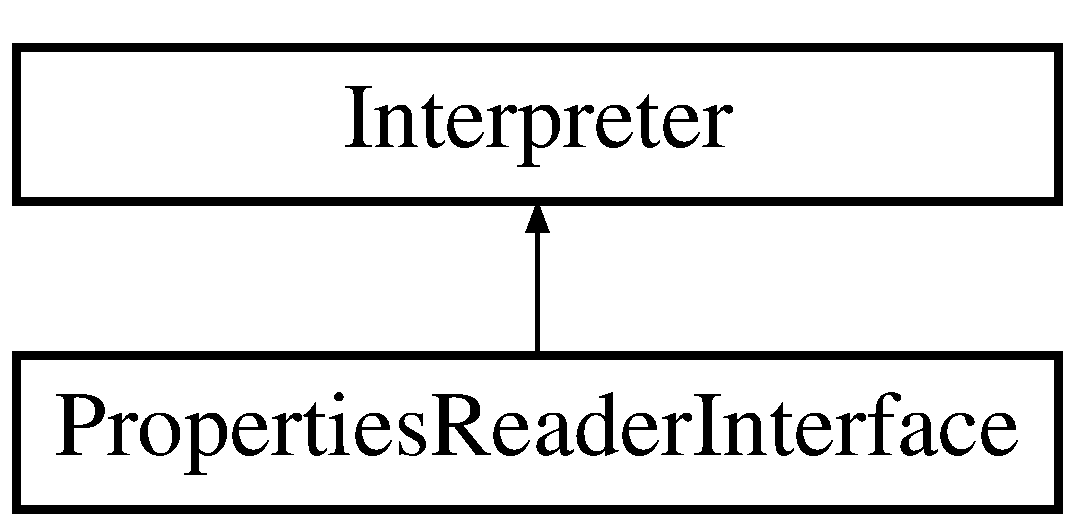
\includegraphics[height=2.000000cm]{classPropertiesReaderInterface}
\end{center}
\end{figure}
\subsection*{Public Member Functions}
\begin{DoxyCompactItemize}
\item 
\hypertarget{classPropertiesReaderInterface_a092db49483a5f97b1eb6e2fdca5b97fb}{virtual bool \hyperlink{classPropertiesReaderInterface_a092db49483a5f97b1eb6e2fdca5b97fb}{opt\-\_\-exist} (std\-::string key)=0}\label{classPropertiesReaderInterface_a092db49483a5f97b1eb6e2fdca5b97fb}

\begin{DoxyCompactList}\small\item\em Does a key exist? \end{DoxyCompactList}\item 
\hypertarget{classPropertiesReaderInterface_a16db6a1917d0274811a499b2a270679b}{virtual std\-::string \hyperlink{classPropertiesReaderInterface_a16db6a1917d0274811a499b2a270679b}{get\-\_\-opt} (std\-::string key)=0}\label{classPropertiesReaderInterface_a16db6a1917d0274811a499b2a270679b}

\begin{DoxyCompactList}\small\item\em Get an option by key. \end{DoxyCompactList}\item 
\hypertarget{classPropertiesReaderInterface_ab088ce690f3f96b3f885d762289c23c2}{virtual bool {\bfseries list\-\_\-exist} (std\-::string key)=0}\label{classPropertiesReaderInterface_ab088ce690f3f96b3f885d762289c23c2}

\item 
\hypertarget{classPropertiesReaderInterface_a466f88254dc3f26691e73ba739bdabce}{virtual std\-::vector$<$ std\-::string $>$ {\bfseries get\-\_\-list} (std\-::string key)=0}\label{classPropertiesReaderInterface_a466f88254dc3f26691e73ba739bdabce}

\end{DoxyCompactItemize}


\subsection{Detailed Description}
\hyperlink{classPropertiesReaderInterface}{Properties\-Reader\-Interface}. 

Here we create a new interpreter by passing in a single argument, the address of a properties file. This file is opened and read, with properties in the form\-: property\-\_\-name=property\-\_\-value This also accepts lists in the form -\/list\-\_\-name-\/list\-\_\-value -\/list\-\_\-name-\/list\-\_\-value2 

The documentation for this class was generated from the following file\-:\begin{DoxyCompactItemize}
\item 
lib/include/factory/properties\-\_\-reader\-\_\-interface.\-h\end{DoxyCompactItemize}

\hypertarget{structRedisConnChain}{\section{Redis\-Conn\-Chain Struct Reference}
\label{structRedisConnChain}\index{Redis\-Conn\-Chain@{Redis\-Conn\-Chain}}
}


A Structure for storing Redis Connection Information.  




{\ttfamily \#include $<$redis\-\_\-interface.\-h$>$}

\subsection*{Public Attributes}
\begin{DoxyCompactItemize}
\item 
\hypertarget{structRedisConnChain_a4694dc63aa9ea1864ddd3bd32324a517}{std\-::string {\bfseries ip}}\label{structRedisConnChain_a4694dc63aa9ea1864ddd3bd32324a517}

\item 
\hypertarget{structRedisConnChain_a5cc9c60a354a6519ab6738a97a30acf9}{int {\bfseries port}}\label{structRedisConnChain_a5cc9c60a354a6519ab6738a97a30acf9}

\item 
\hypertarget{structRedisConnChain_a8bbae840be9aab68e4c98f813915b44c}{std\-::string {\bfseries password}}\label{structRedisConnChain_a8bbae840be9aab68e4c98f813915b44c}

\item 
\hypertarget{structRedisConnChain_a9d8d3258596c3de62a7a71207df2617f}{int {\bfseries pool\-\_\-size}}\label{structRedisConnChain_a9d8d3258596c3de62a7a71207df2617f}

\item 
\hypertarget{structRedisConnChain_aa8503e6bf1350950dda24ad76cd48e24}{int {\bfseries timeout}}\label{structRedisConnChain_aa8503e6bf1350950dda24ad76cd48e24}

\item 
\hypertarget{structRedisConnChain_a92766bf2d64183f8e56515302215b4be}{int {\bfseries role}}\label{structRedisConnChain_a92766bf2d64183f8e56515302215b4be}

\end{DoxyCompactItemize}


\subsection{Detailed Description}
A Structure for storing Redis Connection Information. 

The documentation for this struct was generated from the following file\-:\begin{DoxyCompactItemize}
\item 
lib/include/factory/redis\-\_\-interface.\-h\end{DoxyCompactItemize}

\hypertarget{structRedisConnectionException}{\section{Redis\-Connection\-Exception Struct Reference}
\label{structRedisConnectionException}\index{Redis\-Connection\-Exception@{Redis\-Connection\-Exception}}
}


An Implementation of std\-::exception that denotes a connection error within Redis.  




{\ttfamily \#include $<$redis\-\_\-interface.\-h$>$}

Inheritance diagram for Redis\-Connection\-Exception\-:\begin{figure}[H]
\begin{center}
\leavevmode
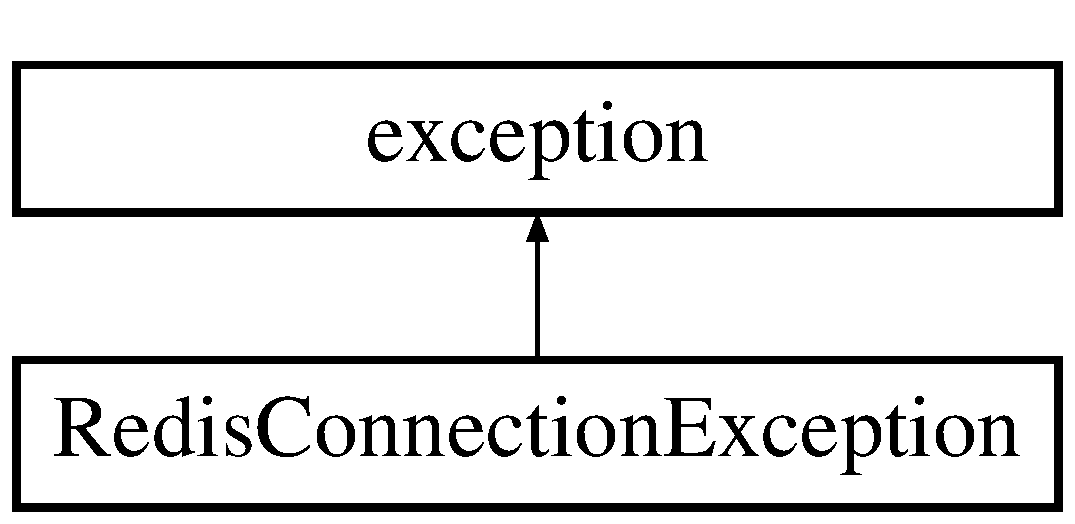
\includegraphics[height=2.000000cm]{structRedisConnectionException}
\end{center}
\end{figure}
\subsection*{Public Member Functions}
\begin{DoxyCompactItemize}
\item 
\hypertarget{structRedisConnectionException_a1a28a564f37ca6c032222fc57611fe7d}{\hyperlink{structRedisConnectionException_a1a28a564f37ca6c032222fc57611fe7d}{Redis\-Connection\-Exception} (std\-::string msg)}\label{structRedisConnectionException_a1a28a564f37ca6c032222fc57611fe7d}

\begin{DoxyCompactList}\small\item\em Create a Redis Connection Exception, and store the given error message. \end{DoxyCompactList}\item 
\hypertarget{structRedisConnectionException_a5af84b976ba7c84d4891c8b42d0c0b34}{\hyperlink{structRedisConnectionException_a5af84b976ba7c84d4891c8b42d0c0b34}{Redis\-Connection\-Exception} (const char $\ast$msg\-\_\-cstr)}\label{structRedisConnectionException_a5af84b976ba7c84d4891c8b42d0c0b34}

\begin{DoxyCompactList}\small\item\em Create a Redis Connection Exception, and store the given error message. \end{DoxyCompactList}\item 
\hypertarget{structRedisConnectionException_a309897cb6e68eea573b2db478543cb16}{const char $\ast$ \hyperlink{structRedisConnectionException_a309897cb6e68eea573b2db478543cb16}{what} () const   throw ()}\label{structRedisConnectionException_a309897cb6e68eea573b2db478543cb16}

\begin{DoxyCompactList}\small\item\em Show the error message in readable format. \end{DoxyCompactList}\end{DoxyCompactItemize}
\subsection*{Public Attributes}
\begin{DoxyCompactItemize}
\item 
\hypertarget{structRedisConnectionException_a95af5cf7df2c6dda75b37574a6cafba4}{std\-::string \hyperlink{structRedisConnectionException_a95af5cf7df2c6dda75b37574a6cafba4}{int\-\_\-msg}}\label{structRedisConnectionException_a95af5cf7df2c6dda75b37574a6cafba4}

\begin{DoxyCompactList}\small\item\em An error message passed on initialization. \end{DoxyCompactList}\end{DoxyCompactItemize}


\subsection{Detailed Description}
An Implementation of std\-::exception that denotes a connection error within Redis. 

The documentation for this struct was generated from the following file\-:\begin{DoxyCompactItemize}
\item 
lib/include/factory/redis\-\_\-interface.\-h\end{DoxyCompactItemize}

\hypertarget{classRedisInterface}{\section{Redis\-Interface Class Reference}
\label{classRedisInterface}\index{Redis\-Interface@{Redis\-Interface}}
}


The X\-Redis Admin.  




{\ttfamily \#include $<$redis\-\_\-interface.\-h$>$}

Inheritance diagram for Redis\-Interface\-:\begin{figure}[H]
\begin{center}
\leavevmode
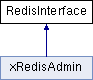
\includegraphics[height=2.000000cm]{classRedisInterface}
\end{center}
\end{figure}
\subsection*{Public Member Functions}
\begin{DoxyCompactItemize}
\item 
\hypertarget{classRedisInterface_afd325866fd98ca6e002b2702e5566ee5}{virtual std\-::string \hyperlink{classRedisInterface_afd325866fd98ca6e002b2702e5566ee5}{load} (const char $\ast$key)=0}\label{classRedisInterface_afd325866fd98ca6e002b2702e5566ee5}

\begin{DoxyCompactList}\small\item\em Load a value from Redis. \end{DoxyCompactList}\item 
\hypertarget{classRedisInterface_adb0d6e3f8a0848cbb6b346e57aeb3ad5}{virtual bool \hyperlink{classRedisInterface_adb0d6e3f8a0848cbb6b346e57aeb3ad5}{save} (const char $\ast$key, std\-::string msg)=0}\label{classRedisInterface_adb0d6e3f8a0848cbb6b346e57aeb3ad5}

\begin{DoxyCompactList}\small\item\em Save a value to Redis. \end{DoxyCompactList}\item 
\hypertarget{classRedisInterface_a3881f54b919852b7aaa231015775544e}{virtual bool \hyperlink{classRedisInterface_a3881f54b919852b7aaa231015775544e}{exists} (const char $\ast$key)=0}\label{classRedisInterface_a3881f54b919852b7aaa231015775544e}

\begin{DoxyCompactList}\small\item\em Does a key exist in Redis? \end{DoxyCompactList}\item 
\hypertarget{classRedisInterface_abb9b1fe2c11911648d62d431968fa04e}{virtual bool \hyperlink{classRedisInterface_abb9b1fe2c11911648d62d431968fa04e}{del} (const char $\ast$key)=0}\label{classRedisInterface_abb9b1fe2c11911648d62d431968fa04e}

\begin{DoxyCompactList}\small\item\em Delete a value from Redis. \end{DoxyCompactList}\item 
\hypertarget{classRedisInterface_ac327841b5c3d227be88f164495e32dd0}{virtual bool \hyperlink{classRedisInterface_ac327841b5c3d227be88f164495e32dd0}{expire} (const char $\ast$key, unsigned int second)=0}\label{classRedisInterface_ac327841b5c3d227be88f164495e32dd0}

\begin{DoxyCompactList}\small\item\em Expire a value in Redis after a specified number of seconds. \end{DoxyCompactList}\end{DoxyCompactItemize}


\subsection{Detailed Description}
The X\-Redis Admin. 

The X\-Redis Admin is responsible for all interactions with the Redis Key-\/\-Value Store. This is capable of connecting to single Redis instances or Clusters 

The documentation for this class was generated from the following file\-:\begin{DoxyCompactItemize}
\item 
lib/include/factory/redis\-\_\-interface.\-h\end{DoxyCompactItemize}

\hypertarget{structRedisKvPair}{\section{Redis\-Kv\-Pair Struct Reference}
\label{structRedisKvPair}\index{Redis\-Kv\-Pair@{Redis\-Kv\-Pair}}
}


A Structure for storing a Key-\/\-Value pair, used with batch operations.  




{\ttfamily \#include $<$redis\-\_\-interface.\-h$>$}

\subsection*{Public Attributes}
\begin{DoxyCompactItemize}
\item 
\hypertarget{structRedisKvPair_af3f52908debaab15e1ed092801d9a875}{std\-::string \hyperlink{structRedisKvPair_af3f52908debaab15e1ed092801d9a875}{key}}\label{structRedisKvPair_af3f52908debaab15e1ed092801d9a875}

\begin{DoxyCompactList}\small\item\em Key of the pair. \end{DoxyCompactList}\item 
\hypertarget{structRedisKvPair_a4d376aa2e230347adc28ac942e3da043}{std\-::string \hyperlink{structRedisKvPair_a4d376aa2e230347adc28ac942e3da043}{val}}\label{structRedisKvPair_a4d376aa2e230347adc28ac942e3da043}

\begin{DoxyCompactList}\small\item\em Value stored in the pair. \end{DoxyCompactList}\end{DoxyCompactItemize}


\subsection{Detailed Description}
A Structure for storing a Key-\/\-Value pair, used with batch operations. 

The documentation for this struct was generated from the following file\-:\begin{DoxyCompactItemize}
\item 
lib/include/factory/redis\-\_\-interface.\-h\end{DoxyCompactItemize}

\hypertarget{structRedisOperationException}{}\section{Redis\+Operation\+Exception Struct Reference}
\label{structRedisOperationException}\index{Redis\+Operation\+Exception@{Redis\+Operation\+Exception}}


An Implementation of std\+::exception that denotes an error within Redis during a transaction.  




{\ttfamily \#include $<$redis\+\_\+interface.\+h$>$}



Inheritance diagram for Redis\+Operation\+Exception\+:
\nopagebreak
\begin{figure}[H]
\begin{center}
\leavevmode
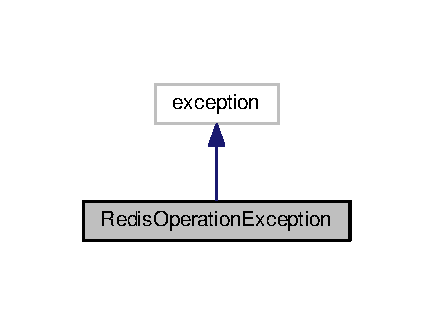
\includegraphics[width=208pt]{structRedisOperationException__inherit__graph}
\end{center}
\end{figure}


Collaboration diagram for Redis\+Operation\+Exception\+:
\nopagebreak
\begin{figure}[H]
\begin{center}
\leavevmode
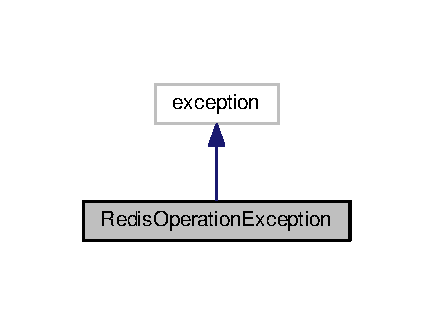
\includegraphics[width=208pt]{structRedisOperationException__coll__graph}
\end{center}
\end{figure}
\subsection*{Public Member Functions}
\begin{DoxyCompactItemize}
\item 
\hyperlink{structRedisOperationException_a54e07b6a7c4d81ab0cb4d1f61d5a6226}{Redis\+Operation\+Exception} (std\+::string msg)\hypertarget{structRedisOperationException_a54e07b6a7c4d81ab0cb4d1f61d5a6226}{}\label{structRedisOperationException_a54e07b6a7c4d81ab0cb4d1f61d5a6226}

\begin{DoxyCompactList}\small\item\em Create a Redis Operation Exception, and store the given error message. \end{DoxyCompactList}\item 
\hyperlink{structRedisOperationException_a330513962eb439159cf494f3996edc8c}{Redis\+Operation\+Exception} (const char $\ast$msg\+\_\+cstr)\hypertarget{structRedisOperationException_a330513962eb439159cf494f3996edc8c}{}\label{structRedisOperationException_a330513962eb439159cf494f3996edc8c}

\begin{DoxyCompactList}\small\item\em Create a Redis Operation Exception, and store the given error message. \end{DoxyCompactList}\item 
const char $\ast$ \hyperlink{structRedisOperationException_a629e013517496f9e14ae5286a8759043}{what} () const   throw ()\hypertarget{structRedisOperationException_a629e013517496f9e14ae5286a8759043}{}\label{structRedisOperationException_a629e013517496f9e14ae5286a8759043}

\begin{DoxyCompactList}\small\item\em Show the error message in readable format. \end{DoxyCompactList}\end{DoxyCompactItemize}
\subsection*{Public Attributes}
\begin{DoxyCompactItemize}
\item 
std\+::string \hyperlink{structRedisOperationException_ac5deeab2028bb95e7db928cfb222656e}{int\+\_\+msg}\hypertarget{structRedisOperationException_ac5deeab2028bb95e7db928cfb222656e}{}\label{structRedisOperationException_ac5deeab2028bb95e7db928cfb222656e}

\begin{DoxyCompactList}\small\item\em An error message passed on initialization. \end{DoxyCompactList}\end{DoxyCompactItemize}


\subsection{Detailed Description}
An Implementation of std\+::exception that denotes an error within Redis during a transaction. 

The documentation for this struct was generated from the following file\+:\begin{DoxyCompactItemize}
\item 
aossl/redis/include/redis\+\_\+interface.\+h\end{DoxyCompactItemize}

\hypertarget{structRequest}{\section{Request Struct Reference}
\label{structRequest}\index{Request@{Request}}
}


A struct that gets passed to callbacks.  




{\ttfamily \#include $<$callbacks.\-h$>$}

\subsection*{Public Member Functions}
\begin{DoxyCompactItemize}
\item 
\hypertarget{structRequest_afaf8d8928de7ffff8a3767589489bd33}{\hyperlink{structRequest_afaf8d8928de7ffff8a3767589489bd33}{Request} ()}\label{structRequest_afaf8d8928de7ffff8a3767589489bd33}

\begin{DoxyCompactList}\small\item\em Constructor. \end{DoxyCompactList}\end{DoxyCompactItemize}
\subsection*{Public Attributes}
\begin{DoxyCompactItemize}
\item 
\hypertarget{structRequest_a23538a8fc246ee789a2461b00dcd6066}{std\-::string \hyperlink{structRequest_a23538a8fc246ee789a2461b00dcd6066}{req\-\_\-data}}\label{structRequest_a23538a8fc246ee789a2461b00dcd6066}

\begin{DoxyCompactList}\small\item\em Used to store original request data. \end{DoxyCompactList}\item 
\hypertarget{structRequest_a16c4515a69beddf526b19514a1de7ed5}{std\-::string \hyperlink{structRequest_a16c4515a69beddf526b19514a1de7ed5}{req\-\_\-addr}}\label{structRequest_a16c4515a69beddf526b19514a1de7ed5}

\begin{DoxyCompactList}\small\item\em Used to store the address on the original request. \end{DoxyCompactList}\item 
\hypertarget{structRequest_a15581550009936223e514df1a38db44e}{int \hyperlink{structRequest_a15581550009936223e514df1a38db44e}{req\-\_\-type}}\label{structRequest_a15581550009936223e514df1a38db44e}

\begin{DoxyCompactList}\small\item\em Used to store the request type. \end{DoxyCompactList}\item 
\hypertarget{structRequest_a9998a7dab5f0eeac6dd70d1f3bf529e3}{\hyperlink{structRequestError}{Request\-Error} $\ast$ \hyperlink{structRequest_a9998a7dab5f0eeac6dd70d1f3bf529e3}{req\-\_\-err}}\label{structRequest_a9998a7dab5f0eeac6dd70d1f3bf529e3}

\begin{DoxyCompactList}\small\item\em Used to store any error messages from the request. \end{DoxyCompactList}\item 
\hypertarget{structRequest_a396a206a5029d7cd8d8f34e1d33c027a}{std\-::string \hyperlink{structRequest_a396a206a5029d7cd8d8f34e1d33c027a}{resp\-\_\-data}}\label{structRequest_a396a206a5029d7cd8d8f34e1d33c027a}

\begin{DoxyCompactList}\small\item\em Used to store response data from the request. \end{DoxyCompactList}\end{DoxyCompactItemize}


\subsection{Detailed Description}
A struct that gets passed to callbacks. 

The documentation for this struct was generated from the following file\-:\begin{DoxyCompactItemize}
\item 
lib/include/factory/callbacks.\-h\end{DoxyCompactItemize}

\hypertarget{structRequestError}{\section{Request\-Error Struct Reference}
\label{structRequestError}\index{Request\-Error@{Request\-Error}}
}


A struct that gets passed to callbacks to transmit errors.  




{\ttfamily \#include $<$callbacks.\-h$>$}

\subsection*{Public Attributes}
\begin{DoxyCompactItemize}
\item 
\hypertarget{structRequestError_abb80687d9ab9393139a6591b71248f4f}{int \hyperlink{structRequestError_abb80687d9ab9393139a6591b71248f4f}{err\-\_\-code}}\label{structRequestError_abb80687d9ab9393139a6591b71248f4f}

\begin{DoxyCompactList}\small\item\em A numerical error code. \end{DoxyCompactList}\item 
\hypertarget{structRequestError_a6d14b796dda607dfd6e0c6736f9dec96}{std\-::string \hyperlink{structRequestError_a6d14b796dda607dfd6e0c6736f9dec96}{err\-\_\-message}}\label{structRequestError_a6d14b796dda607dfd6e0c6736f9dec96}

\begin{DoxyCompactList}\small\item\em An Error message. \end{DoxyCompactList}\end{DoxyCompactItemize}


\subsection{Detailed Description}
A struct that gets passed to callbacks to transmit errors. 

The documentation for this struct was generated from the following file\-:\begin{DoxyCompactItemize}
\item 
lib/include/factory/callbacks.\-h\end{DoxyCompactItemize}

\hypertarget{classResultsIteratorInterface}{\section{Results\-Iterator\-Interface Class Reference}
\label{classResultsIteratorInterface}\index{Results\-Iterator\-Interface@{Results\-Iterator\-Interface}}
}


Results Iterator for viewing query results.  




{\ttfamily \#include $<$neo4j\-\_\-interface.\-h$>$}

\subsection*{Public Member Functions}
\begin{DoxyCompactItemize}
\item 
\hypertarget{classResultsIteratorInterface_a4f6574b8a57dbd2ea3c86e66bf260252}{virtual void \hyperlink{classResultsIteratorInterface_a4f6574b8a57dbd2ea3c86e66bf260252}{clear} ()=0}\label{classResultsIteratorInterface_a4f6574b8a57dbd2ea3c86e66bf260252}

\begin{DoxyCompactList}\small\item\em Clear the results iterator of all values. \end{DoxyCompactList}\item 
virtual bool \hyperlink{classResultsIteratorInterface_ab00e99e5bd9f186eb9bdcdf30d594b99}{empty} ()=0
\begin{DoxyCompactList}\small\item\em Is the iterator empty? \end{DoxyCompactList}\item 
\hypertarget{classResultsIteratorInterface_a9a022aba2a3e7771c8d147885ca151dd}{virtual unsigned int \hyperlink{classResultsIteratorInterface_a9a022aba2a3e7771c8d147885ca151dd}{length} ()=0}\label{classResultsIteratorInterface_a9a022aba2a3e7771c8d147885ca151dd}

\begin{DoxyCompactList}\small\item\em Get the number of results in the query. \end{DoxyCompactList}\item 
\hypertarget{classResultsIteratorInterface_a00385bfa8ddabb267cf46006a9a0f6e9}{virtual \hyperlink{classResultTreeInterface}{Result\-Tree\-Interface} $\ast$ \hyperlink{classResultsIteratorInterface_a00385bfa8ddabb267cf46006a9a0f6e9}{next} ()=0}\label{classResultsIteratorInterface_a00385bfa8ddabb267cf46006a9a0f6e9}

\begin{DoxyCompactList}\small\item\em Get the next query result. \end{DoxyCompactList}\end{DoxyCompactItemize}


\subsection{Detailed Description}
Results Iterator for viewing query results. 

Accepts a result stream as an input, returns Results Trees for each entry that matches in the query Deletes it when finished 

\subsection{Member Function Documentation}
\hypertarget{classResultsIteratorInterface_ab00e99e5bd9f186eb9bdcdf30d594b99}{\index{Results\-Iterator\-Interface@{Results\-Iterator\-Interface}!empty@{empty}}
\index{empty@{empty}!ResultsIteratorInterface@{Results\-Iterator\-Interface}}
\subsubsection[{empty}]{\setlength{\rightskip}{0pt plus 5cm}virtual bool Results\-Iterator\-Interface\-::empty (
\begin{DoxyParamCaption}
{}
\end{DoxyParamCaption}
)\hspace{0.3cm}{\ttfamily [pure virtual]}}}\label{classResultsIteratorInterface_ab00e99e5bd9f186eb9bdcdf30d594b99}


Is the iterator empty? 

Return true if this iterator contains no results. Return false otherwise. 

The documentation for this class was generated from the following file\-:\begin{DoxyCompactItemize}
\item 
lib/include/factory/neo4j\-\_\-interface.\-h\end{DoxyCompactItemize}

\hypertarget{classResultTreeInterface}{\section{Result\-Tree\-Interface Class Reference}
\label{classResultTreeInterface}\index{Result\-Tree\-Interface@{Result\-Tree\-Interface}}
}


Tree of Query Results.  




{\ttfamily \#include $<$neo4j\-\_\-interface.\-h$>$}

\subsection*{Public Member Functions}
\begin{DoxyCompactItemize}
\item 
\hypertarget{classResultTreeInterface_acc4e0493661f5f2b0b836c7a1bdb3a8f}{virtual \hyperlink{classDbObjectInterface}{Db\-Object\-Interface} $\ast$ \hyperlink{classResultTreeInterface_acc4e0493661f5f2b0b836c7a1bdb3a8f}{get} (int index)=0}\label{classResultTreeInterface_acc4e0493661f5f2b0b836c7a1bdb3a8f}

\begin{DoxyCompactList}\small\item\em Get the node/edge at the specified index. \end{DoxyCompactList}\end{DoxyCompactItemize}


\subsection{Detailed Description}
Tree of Query Results. 

The documentation for this class was generated from the following file\-:\begin{DoxyCompactItemize}
\item 
lib/include/factory/neo4j\-\_\-interface.\-h\end{DoxyCompactItemize}

\hypertarget{classServiceInterface}{}\section{Service\+Interface Class Reference}
\label{classServiceInterface}\index{Service\+Interface@{Service\+Interface}}


A Service class which can be registered with Consul for each instance of a particular service.  




{\ttfamily \#include $<$consul\+\_\+interface.\+h$>$}

\subsection*{Public Member Functions}
\begin{DoxyCompactItemize}
\item 
virtual std\+::string \hyperlink{classServiceInterface_a2c041d65d3e725f1cf8e2379f4620d58}{to\+\_\+json} ()=0
\begin{DoxyCompactList}\small\item\em Convert the Service into a J\+S\+ON Message. \end{DoxyCompactList}\item 
virtual std\+::string \hyperlink{classServiceInterface_a0ba731e4d379cbeddc852304b470c617}{get\+\_\+id} ()=0\hypertarget{classServiceInterface_a0ba731e4d379cbeddc852304b470c617}{}\label{classServiceInterface_a0ba731e4d379cbeddc852304b470c617}

\begin{DoxyCompactList}\small\item\em Get the Service ID. \end{DoxyCompactList}\item 
virtual std\+::string \hyperlink{classServiceInterface_aed2140959e23f98cd0cca1a101646384}{get\+\_\+name} ()=0\hypertarget{classServiceInterface_aed2140959e23f98cd0cca1a101646384}{}\label{classServiceInterface_aed2140959e23f98cd0cca1a101646384}

\begin{DoxyCompactList}\small\item\em Get the Service Name. \end{DoxyCompactList}\item 
virtual std\+::string \hyperlink{classServiceInterface_a6c4fd6eff9e1c8eed5dfed301d2f8047}{get\+\_\+address} ()=0\hypertarget{classServiceInterface_a6c4fd6eff9e1c8eed5dfed301d2f8047}{}\label{classServiceInterface_a6c4fd6eff9e1c8eed5dfed301d2f8047}

\begin{DoxyCompactList}\small\item\em Get the Service Address. \end{DoxyCompactList}\item 
virtual std\+::string \hyperlink{classServiceInterface_a7c8a328711f7fb019a9f7dadcb897cb0}{get\+\_\+port} ()=0\hypertarget{classServiceInterface_a7c8a328711f7fb019a9f7dadcb897cb0}{}\label{classServiceInterface_a7c8a328711f7fb019a9f7dadcb897cb0}

\begin{DoxyCompactList}\small\item\em Get the Service Port. \end{DoxyCompactList}\item 
virtual void \hyperlink{classServiceInterface_aade793bb679fa00cd34194a3623c554a}{set\+\_\+id} (std\+::string new\+\_\+id)=0\hypertarget{classServiceInterface_aade793bb679fa00cd34194a3623c554a}{}\label{classServiceInterface_aade793bb679fa00cd34194a3623c554a}

\begin{DoxyCompactList}\small\item\em Set the Service ID. \end{DoxyCompactList}\item 
virtual void \hyperlink{classServiceInterface_ac9b2d1a785b665ef3c575f5877148511}{set\+\_\+name} (std\+::string new\+\_\+name)=0\hypertarget{classServiceInterface_ac9b2d1a785b665ef3c575f5877148511}{}\label{classServiceInterface_ac9b2d1a785b665ef3c575f5877148511}

\begin{DoxyCompactList}\small\item\em Set the Service Name. \end{DoxyCompactList}\item 
virtual void \hyperlink{classServiceInterface_a619fb75631f816d547d2ad3efeae2bf5}{set\+\_\+address} (std\+::string new\+\_\+address)=0\hypertarget{classServiceInterface_a619fb75631f816d547d2ad3efeae2bf5}{}\label{classServiceInterface_a619fb75631f816d547d2ad3efeae2bf5}

\begin{DoxyCompactList}\small\item\em Set the Service Address. \end{DoxyCompactList}\item 
virtual void \hyperlink{classServiceInterface_a2c9385fbc567949560dc7972e6a7059e}{set\+\_\+port} (std\+::string new\+\_\+port)=0\hypertarget{classServiceInterface_a2c9385fbc567949560dc7972e6a7059e}{}\label{classServiceInterface_a2c9385fbc567949560dc7972e6a7059e}

\begin{DoxyCompactList}\small\item\em Set the Service Port. \end{DoxyCompactList}\item 
virtual std\+::vector$<$ std\+::string $>$ \hyperlink{classServiceInterface_afdc1ce12ef5ff09cf82e3d0f8ea7724a}{get\+\_\+tags} ()=0\hypertarget{classServiceInterface_afdc1ce12ef5ff09cf82e3d0f8ea7724a}{}\label{classServiceInterface_afdc1ce12ef5ff09cf82e3d0f8ea7724a}

\begin{DoxyCompactList}\small\item\em Get the tags. \end{DoxyCompactList}\item 
virtual void \hyperlink{classServiceInterface_ac8b80c9301fa04ea295acecd88b9cc42}{add\+\_\+tag} (std\+::string new\+\_\+tag)=0\hypertarget{classServiceInterface_ac8b80c9301fa04ea295acecd88b9cc42}{}\label{classServiceInterface_ac8b80c9301fa04ea295acecd88b9cc42}

\begin{DoxyCompactList}\small\item\em Add a tag. \end{DoxyCompactList}\item 
virtual void \hyperlink{classServiceInterface_a3e27c216421be0e92984b07a095f1279}{clear\+\_\+tags} ()=0\hypertarget{classServiceInterface_a3e27c216421be0e92984b07a095f1279}{}\label{classServiceInterface_a3e27c216421be0e92984b07a095f1279}

\begin{DoxyCompactList}\small\item\em Clear the tags. \end{DoxyCompactList}\item 
virtual int \hyperlink{classServiceInterface_aad0434e39242a47048659a1243fab46e}{num\+\_\+tags} () const =0\hypertarget{classServiceInterface_aad0434e39242a47048659a1243fab46e}{}\label{classServiceInterface_aad0434e39242a47048659a1243fab46e}

\begin{DoxyCompactList}\small\item\em How many tags are there? \end{DoxyCompactList}\item 
virtual \hyperlink{structHealthCheck}{Health\+Check} \hyperlink{classServiceInterface_afa5e0a43120dcd89dfcf7ae8aa086217}{get\+\_\+check} ()=0\hypertarget{classServiceInterface_afa5e0a43120dcd89dfcf7ae8aa086217}{}\label{classServiceInterface_afa5e0a43120dcd89dfcf7ae8aa086217}

\begin{DoxyCompactList}\small\item\em Get the health checks. \end{DoxyCompactList}\item 
virtual void \hyperlink{classServiceInterface_a32065df2094fa5a53708f5ff3944195b}{set\+\_\+check} (std\+::string scr, int interval\+\_\+seconds)=0\hypertarget{classServiceInterface_a32065df2094fa5a53708f5ff3944195b}{}\label{classServiceInterface_a32065df2094fa5a53708f5ff3944195b}

\begin{DoxyCompactList}\small\item\em Add a check. \end{DoxyCompactList}\end{DoxyCompactItemize}


\subsection{Detailed Description}
A Service class which can be registered with Consul for each instance of a particular service. 

An instance of this class can be instantiated by a service and is passed to the consul admin to register and de-\/register 

\subsection{Member Function Documentation}
\index{Service\+Interface@{Service\+Interface}!to\+\_\+json@{to\+\_\+json}}
\index{to\+\_\+json@{to\+\_\+json}!Service\+Interface@{Service\+Interface}}
\subsubsection[{\texorpdfstring{to\+\_\+json()=0}{to_json()=0}}]{\setlength{\rightskip}{0pt plus 5cm}virtual std\+::string Service\+Interface\+::to\+\_\+json (
\begin{DoxyParamCaption}
{}
\end{DoxyParamCaption}
)\hspace{0.3cm}{\ttfamily [pure virtual]}}\hypertarget{classServiceInterface_a2c041d65d3e725f1cf8e2379f4620d58}{}\label{classServiceInterface_a2c041d65d3e725f1cf8e2379f4620d58}


Convert the Service into a J\+S\+ON Message. 

Method that allows the service to be transformed into a json message that can be sent via H\+T\+TP to a Consul instance 

The documentation for this class was generated from the following file\+:\begin{DoxyCompactItemize}
\item 
aossl/consul/include/consul\+\_\+interface.\+h\end{DoxyCompactItemize}

\hypertarget{structUuidContainer}{}\section{Uuid\+Container Struct Reference}
\label{structUuidContainer}\index{Uuid\+Container@{Uuid\+Container}}


A return structure which captures any security error messages thrown by the framework.  




{\ttfamily \#include $<$uuid\+\_\+interface.\+h$>$}

\subsection*{Public Attributes}
\begin{DoxyCompactItemize}
\item 
std\+::string \hyperlink{structUuidContainer_aea2f6e3768858acb4086cd1a93c5666a}{id}\hypertarget{structUuidContainer_aea2f6e3768858acb4086cd1a93c5666a}{}\label{structUuidContainer_aea2f6e3768858acb4086cd1a93c5666a}

\begin{DoxyCompactList}\small\item\em The U\+U\+ID generated. \end{DoxyCompactList}\item 
std\+::string \hyperlink{structUuidContainer_a58e21d1df4638157e157a41fa95a5e07}{err}\hypertarget{structUuidContainer_a58e21d1df4638157e157a41fa95a5e07}{}\label{structUuidContainer_a58e21d1df4638157e157a41fa95a5e07}

\begin{DoxyCompactList}\small\item\em Is either empty or contains an error message. \end{DoxyCompactList}\end{DoxyCompactItemize}


\subsection{Detailed Description}
A return structure which captures any security error messages thrown by the framework. 

The documentation for this struct was generated from the following file\+:\begin{DoxyCompactItemize}
\item 
aossl/uuid/include/uuid\+\_\+interface.\+h\end{DoxyCompactItemize}

\hypertarget{classuuidInterface}{\section{uuid\-Interface Class Reference}
\label{classuuidInterface}\index{uuid\-Interface@{uuid\-Interface}}
}


U\-U\-I\-D Admin.  




{\ttfamily \#include $<$uuid\-\_\-interface.\-h$>$}

Inheritance diagram for uuid\-Interface\-:\begin{figure}[H]
\begin{center}
\leavevmode
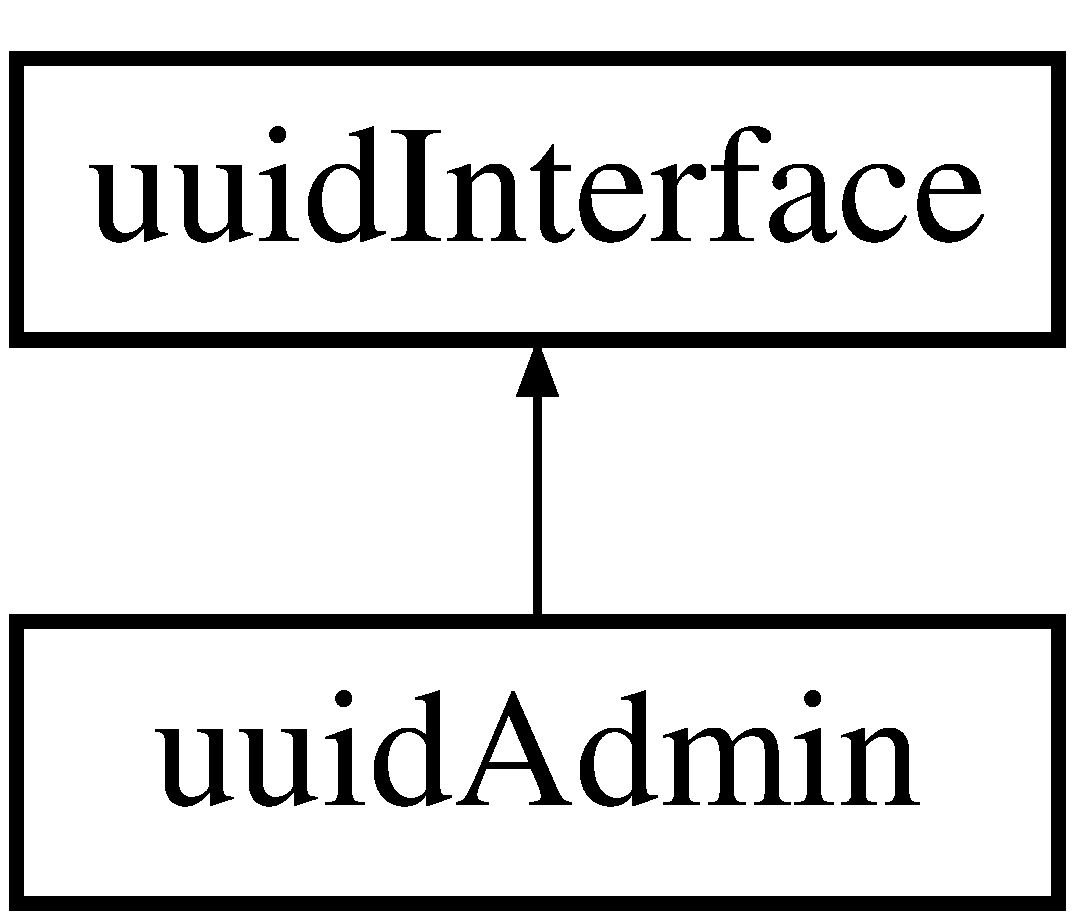
\includegraphics[height=2.000000cm]{classuuidInterface}
\end{center}
\end{figure}
\subsection*{Public Member Functions}
\begin{DoxyCompactItemize}
\item 
virtual std\-::string \hyperlink{classuuidInterface_ae1696692de5b139246154c8d32d44797}{generate} ()=0
\begin{DoxyCompactList}\small\item\em Generate a new U\-U\-I\-D. \end{DoxyCompactList}\end{DoxyCompactItemize}


\subsection{Detailed Description}
U\-U\-I\-D Admin. 

The U\-U\-I\-D Admin is in charge of generating any Universally Unique I\-D's that are required throughout program execution 

\subsection{Member Function Documentation}
\hypertarget{classuuidInterface_ae1696692de5b139246154c8d32d44797}{\index{uuid\-Interface@{uuid\-Interface}!generate@{generate}}
\index{generate@{generate}!uuidInterface@{uuid\-Interface}}
\subsubsection[{generate}]{\setlength{\rightskip}{0pt plus 5cm}virtual std\-::string uuid\-Interface\-::generate (
\begin{DoxyParamCaption}
{}
\end{DoxyParamCaption}
)\hspace{0.3cm}{\ttfamily [pure virtual]}}}\label{classuuidInterface_ae1696692de5b139246154c8d32d44797}


Generate a new U\-U\-I\-D. 

The method will generate on the means of generation present on your system In some cases, this may result in U\-U\-I\-D's being generated that pose a security risk. In this case, that fact will be clearly called out in the logs, and it is recommended that production systems are tested to ensure that U\-U\-I\-D's are generated in a safe manner 

Implemented in \hyperlink{classuuidAdmin_a344f39f4c1e15cf72e64b3544312d7ed}{uuid\-Admin}.



The documentation for this class was generated from the following file\-:\begin{DoxyCompactItemize}
\item 
lib/include/factory/uuid\-\_\-interface.\-h\end{DoxyCompactItemize}

\hypertarget{classZmqIn}{\section{Zmq\-In Class Reference}
\label{classZmqIn}\index{Zmq\-In@{Zmq\-In}}
}


An Inbound Z\-M\-Q Manager.  




{\ttfamily \#include $<$zmq\-\_\-interface.\-h$>$}

Inheritance diagram for Zmq\-In\-:\begin{figure}[H]
\begin{center}
\leavevmode
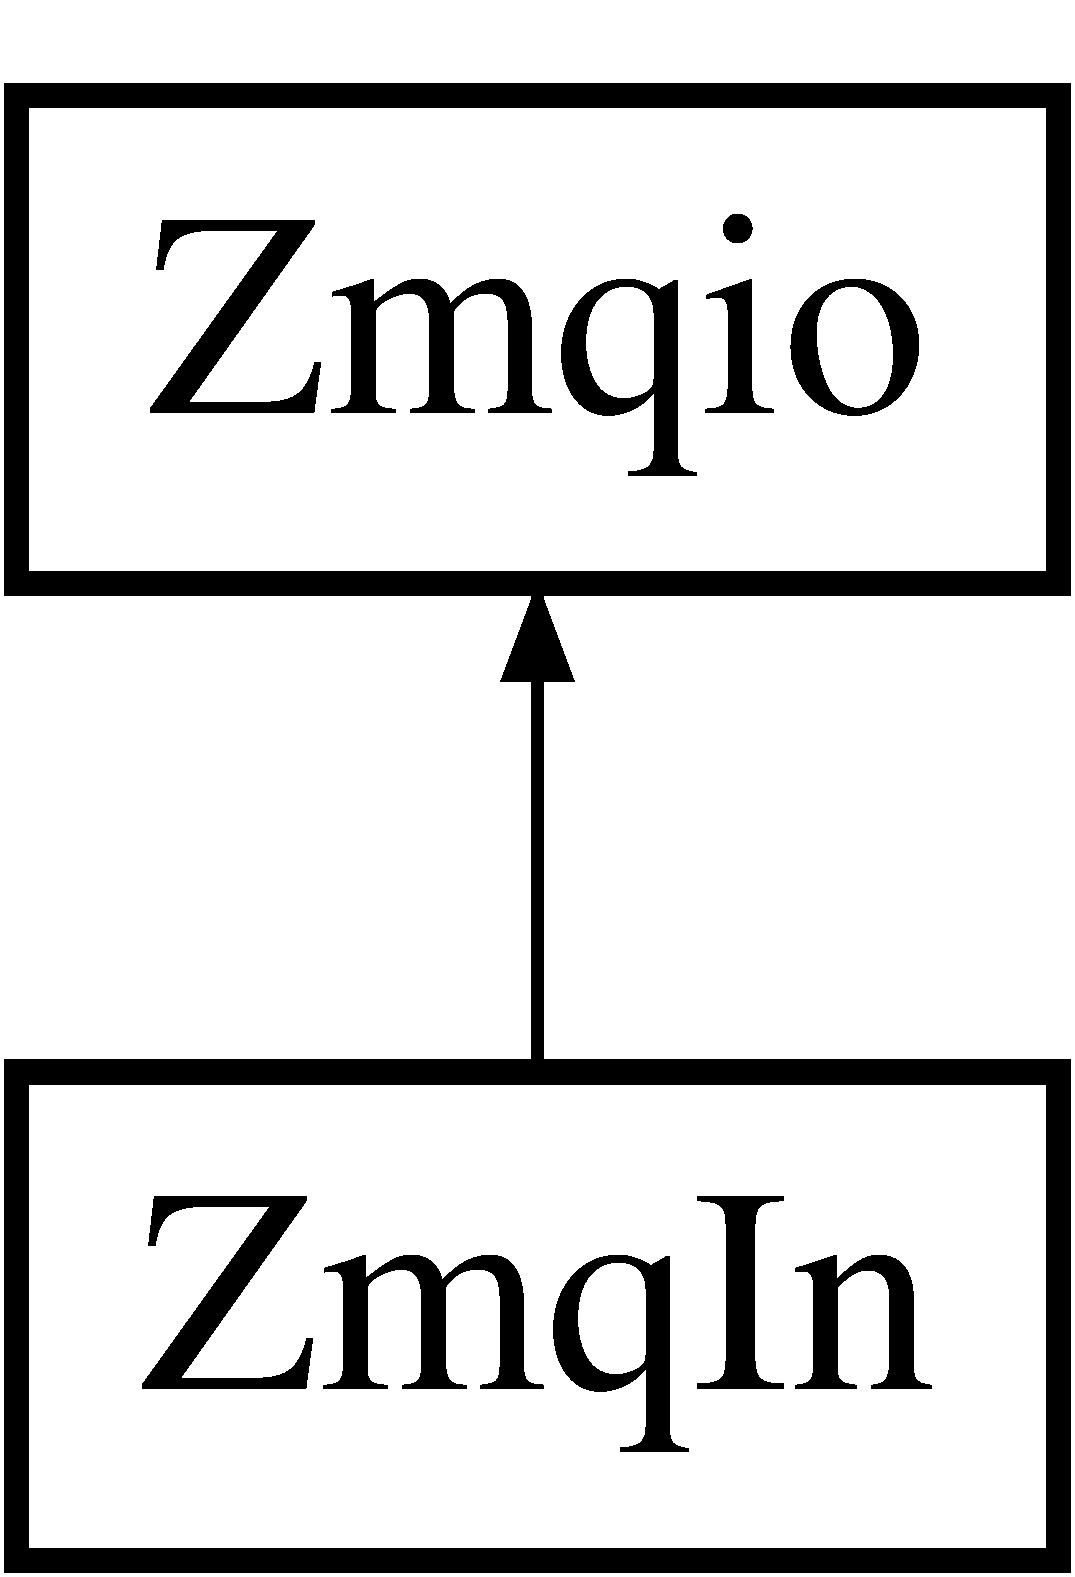
\includegraphics[height=2.000000cm]{classZmqIn}
\end{center}
\end{figure}
\subsection*{Public Member Functions}
\begin{DoxyCompactItemize}
\item 
\hypertarget{classZmqIn_ad6037a187635f7d46bab5da961156751}{virtual void \hyperlink{classZmqIn_ad6037a187635f7d46bab5da961156751}{bind} (std\-::string conn\-\_\-str)=0}\label{classZmqIn_ad6037a187635f7d46bab5da961156751}

\begin{DoxyCompactList}\small\item\em Bind on the given conn\-\_\-str. \end{DoxyCompactList}\item 
\hypertarget{classZmqIn_a375de593defd4c2cf3adebad063950fe}{virtual std\-::string \hyperlink{classZmqIn_a375de593defd4c2cf3adebad063950fe}{recv} ()=0}\label{classZmqIn_a375de593defd4c2cf3adebad063950fe}

\begin{DoxyCompactList}\small\item\em Recieve a message on the port. \end{DoxyCompactList}\item 
\hypertarget{classZmqIn_ad2a35cc76a5b0b2412fda5418f708e60}{virtual void \hyperlink{classZmqIn_ad2a35cc76a5b0b2412fda5418f708e60}{send} (const char $\ast$msg, int msg\-\_\-size)=0}\label{classZmqIn_ad2a35cc76a5b0b2412fda5418f708e60}

\begin{DoxyCompactList}\small\item\em Send a message on the port. \end{DoxyCompactList}\item 
\hypertarget{classZmqIn_adf4165c263ddc5b68099b93b9f37f592}{virtual void \hyperlink{classZmqIn_adf4165c263ddc5b68099b93b9f37f592}{send} (std\-::string msg)=0}\label{classZmqIn_adf4165c263ddc5b68099b93b9f37f592}

\begin{DoxyCompactList}\small\item\em Send a string on the port. \end{DoxyCompactList}\item 
\hypertarget{classZmqIn_a1b7ed3f43e1796a5a0cdd090f69ae932}{virtual void \hyperlink{classZmqIn_a1b7ed3f43e1796a5a0cdd090f69ae932}{subscribe} (std\-::string filter)=0}\label{classZmqIn_a1b7ed3f43e1796a5a0cdd090f69ae932}

\begin{DoxyCompactList}\small\item\em Subscribe on a particular filter (only effective for Pub/\-Sub) \end{DoxyCompactList}\end{DoxyCompactItemize}


\subsection{Detailed Description}
An Inbound Z\-M\-Q Manager. 

Acts as the Responder (Server) in the Z\-M\-Q Sockets Recieve, then Send 

The documentation for this class was generated from the following file\-:\begin{DoxyCompactItemize}
\item 
lib/include/factory/zmq\-\_\-interface.\-h\end{DoxyCompactItemize}

\hypertarget{classZmqio}{\section{Zmqio Class Reference}
\label{classZmqio}\index{Zmqio@{Zmqio}}
}


An Interface for Z\-M\-Q\-I\-O.  




{\ttfamily \#include $<$zmq\-\_\-interface.\-h$>$}

Inheritance diagram for Zmqio\-:\begin{figure}[H]
\begin{center}
\leavevmode
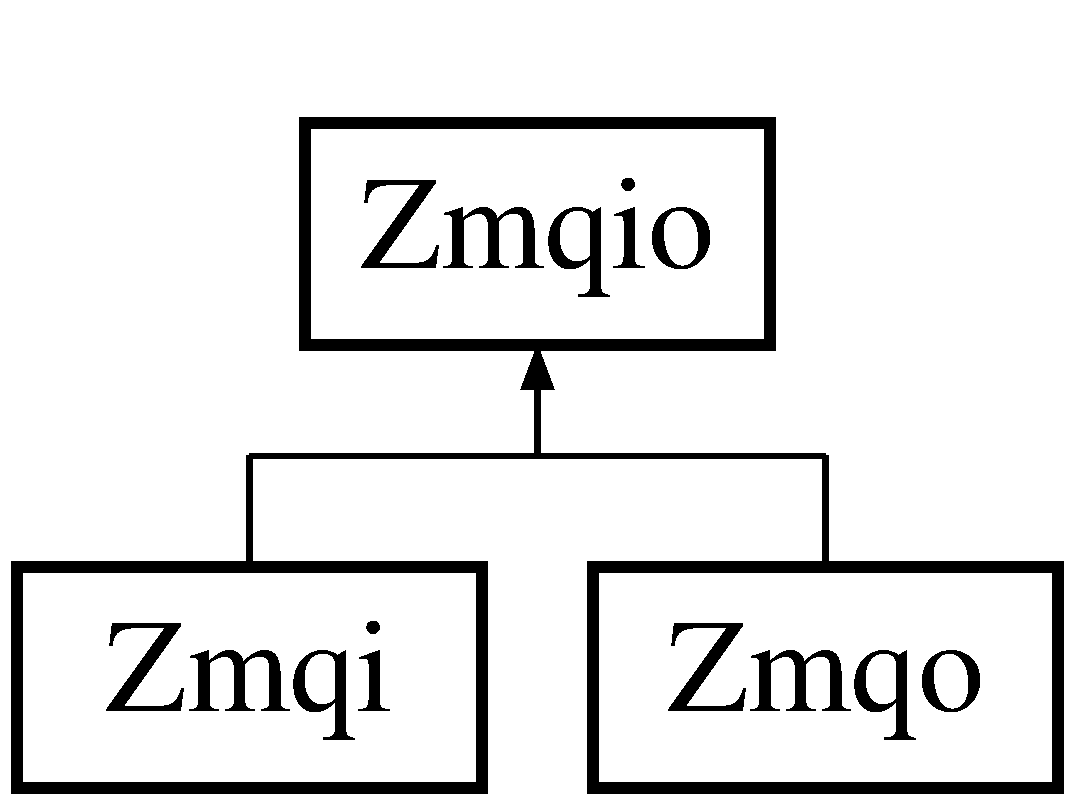
\includegraphics[height=2.000000cm]{classZmqio}
\end{center}
\end{figure}
\subsection*{Public Member Functions}
\begin{DoxyCompactItemize}
\item 
\hypertarget{classZmqio_a9365ac0ed42905898502e16857997acc}{virtual std\-::string \hyperlink{classZmqio_a9365ac0ed42905898502e16857997acc}{recv} ()=0}\label{classZmqio_a9365ac0ed42905898502e16857997acc}

\begin{DoxyCompactList}\small\item\em Recieve a message on the port. \end{DoxyCompactList}\item 
\hypertarget{classZmqio_a858e00e8ac5c4d1d60c665fa7c0716f0}{virtual void \hyperlink{classZmqio_a858e00e8ac5c4d1d60c665fa7c0716f0}{send} (const char $\ast$msg, int msg\-\_\-size)=0}\label{classZmqio_a858e00e8ac5c4d1d60c665fa7c0716f0}

\begin{DoxyCompactList}\small\item\em Send a message on the port. \end{DoxyCompactList}\item 
\hypertarget{classZmqio_a079f5752b553ddb2e5a2da565bcf162c}{virtual void \hyperlink{classZmqio_a079f5752b553ddb2e5a2da565bcf162c}{send} (std\-::string msg)=0}\label{classZmqio_a079f5752b553ddb2e5a2da565bcf162c}

\begin{DoxyCompactList}\small\item\em Send a string on the port. \end{DoxyCompactList}\item 
\hypertarget{classZmqio_aa315934401c5a3ba2eb502c16a3a6aca}{virtual void \hyperlink{classZmqio_aa315934401c5a3ba2eb502c16a3a6aca}{subscribe} (std\-::string filter)=0}\label{classZmqio_aa315934401c5a3ba2eb502c16a3a6aca}

\begin{DoxyCompactList}\small\item\em Subscribe on a particular filter (only effective for Pub/\-Sub) \end{DoxyCompactList}\end{DoxyCompactItemize}


\subsection{Detailed Description}
An Interface for Z\-M\-Q\-I\-O. 

Defines the methods that the Z\-M\-Q Managers must implement send \& recv, as well as subscribe 

The documentation for this class was generated from the following file\-:\begin{DoxyCompactItemize}
\item 
lib/include/factory/zmq\-\_\-interface.\-h\end{DoxyCompactItemize}

\hypertarget{classZmqOut}{\section{Zmq\-Out Class Reference}
\label{classZmqOut}\index{Zmq\-Out@{Zmq\-Out}}
}


An Outbound Z\-M\-Q Manager.  




{\ttfamily \#include $<$zmq\-\_\-interface.\-h$>$}

Inheritance diagram for Zmq\-Out\-:\begin{figure}[H]
\begin{center}
\leavevmode
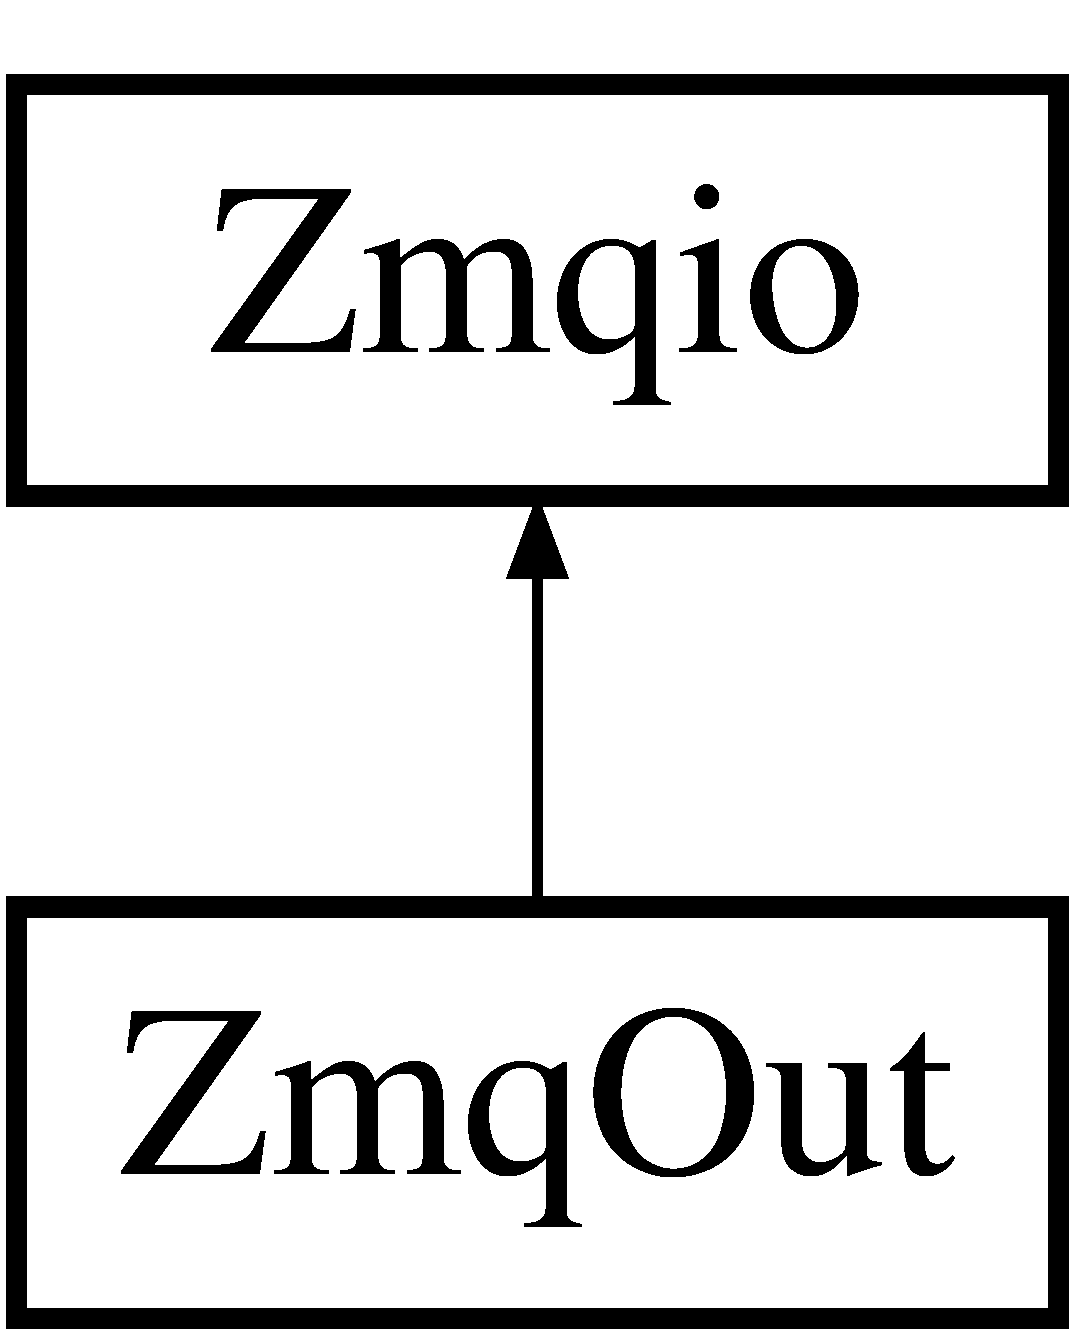
\includegraphics[height=2.000000cm]{classZmqOut}
\end{center}
\end{figure}
\subsection*{Public Member Functions}
\begin{DoxyCompactItemize}
\item 
\hypertarget{classZmqOut_ae34b1742c72e0c82ea42315cb68f1a20}{virtual void \hyperlink{classZmqOut_ae34b1742c72e0c82ea42315cb68f1a20}{connect} (std\-::string conn\-\_\-str)=0}\label{classZmqOut_ae34b1742c72e0c82ea42315cb68f1a20}

\begin{DoxyCompactList}\small\item\em Connect to the given conn\-\_\-str. \end{DoxyCompactList}\item 
\hypertarget{classZmqOut_a97935d9e7cbacd2fcb9655433e4b7af4}{virtual void \hyperlink{classZmqOut_a97935d9e7cbacd2fcb9655433e4b7af4}{send} (const char $\ast$msg, int msg\-\_\-size)=0}\label{classZmqOut_a97935d9e7cbacd2fcb9655433e4b7af4}

\begin{DoxyCompactList}\small\item\em Send a message on the port. \end{DoxyCompactList}\item 
\hypertarget{classZmqOut_ac7b314ddf6e0357c31b05fb2b1b91635}{virtual void \hyperlink{classZmqOut_ac7b314ddf6e0357c31b05fb2b1b91635}{send} (std\-::string msg)=0}\label{classZmqOut_ac7b314ddf6e0357c31b05fb2b1b91635}

\begin{DoxyCompactList}\small\item\em Send a string on the port. \end{DoxyCompactList}\item 
\hypertarget{classZmqOut_a02da5e5dd51f99e7d35a3f843b9bd00e}{virtual std\-::string \hyperlink{classZmqOut_a02da5e5dd51f99e7d35a3f843b9bd00e}{recv} ()=0}\label{classZmqOut_a02da5e5dd51f99e7d35a3f843b9bd00e}

\begin{DoxyCompactList}\small\item\em Recieve a message on the port. \end{DoxyCompactList}\end{DoxyCompactItemize}


\subsection{Detailed Description}
An Outbound Z\-M\-Q Manager. 

Acts as the Requestor (Client) in the Z\-M\-Q Sockets Send, then Recieve 

The documentation for this class was generated from the following file\-:\begin{DoxyCompactItemize}
\item 
lib/include/factory/zmq\-\_\-interface.\-h\end{DoxyCompactItemize}

%--- End generated contents ---

% Index
\newpage
\phantomsection
\addcontentsline{toc}{part}{Index}
\printindex

\end{document}
